\documentclass[twocolumn]{article}

\usepackage{verbatim}
\usepackage{graphicx}
\usepackage{geometry}
\usepackage[firstpage]{draftwatermark}
\usepackage{cuted}
\usepackage{float}
\usepackage{tikz,pgfplots}


\renewcommand{\familydefault}{\sfdefault}

\title{Planned Communities}
\date{2019-02-01}
\author{Tobias Blaser}

\geometry{
	left=2cm,
	top=2cm,
	right=2cm,
	bottom=3cm
}


\begin{document}

	\newgeometry{top=5cm,right=0cm,left=0cm,bottom=2cm}
	\pagenumbering{gobble}
	
	\SetWatermarkScale{0.75}
	\SetWatermarkText{
		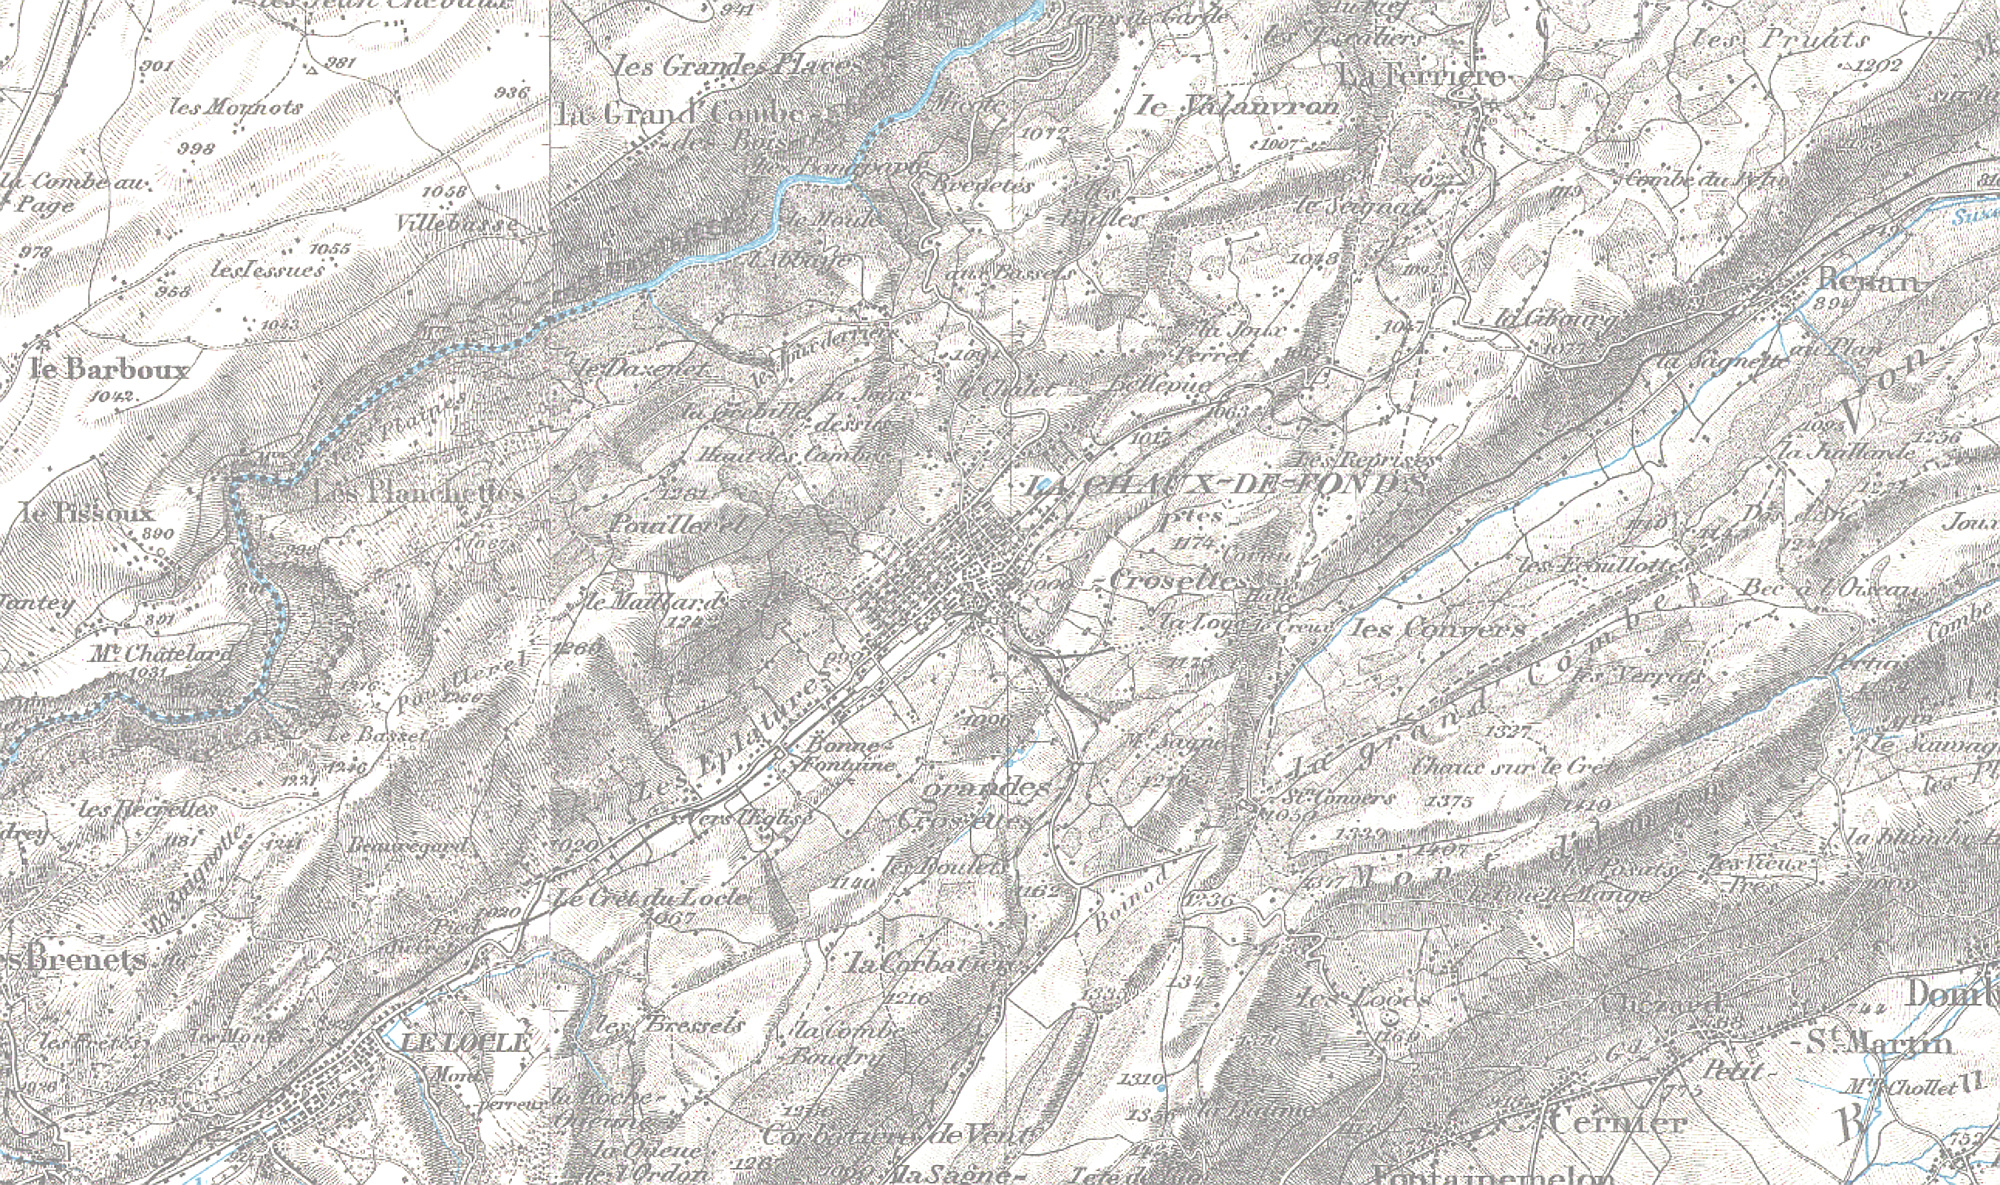
\includegraphics[angle=-45]{images/cover-background.jpg}
	}
	
	\maketitle	
 	
	\begin{figure}[b!]
 		\includegraphics[
 			width=\textwidth,
 			trim={0 1cm 0 1cm},
 			clip
 		]{images/la-chaux-de-fonds/1280px-Rue_du_Progrès_in_La_Chaux-de-Fonds.jpg}
 	\end{figure}
 	
 	\restoregeometry	
	
	
	\clearpage
	\pagenumbering{arabic}
	
	\begin{strip}
	\tableofcontents
	\paragraph{Cover images}
	Map of La Chaux-de-fonds 1920\cite{MapGeoAdmin:LaChauxDeFonds1920},
	Rue du Progrès in La Chaux-de-Fonds\cite{Wikimedia:RueDuProgressLaChauxDeFonds}
	\end{strip}
	
	% TODO page break
	\clearpage
	\section{Summary}
		\subsection{Purpose}
		The purpose of this document, is to compare the growth strategies of planned cities from different countries and centuries.
		The following cities are compared:
		
		\begin{description}
			\item [La Chaux-de-Fonds] Switzerland, Europe, Planned 1794
			\item [La Plata] Argentina, South America, Planned 1882
			\item [Abuja FCT] Nigeria, Africa, Planned 1976
		\end{description}
		La Plata (Argentina), La Chaux-de-Fonds (Switzerland) and Abuja FCT (Nigeria)

		\subsection{Methodology}

		\subsection{Findings}


	\clearpage
	\section{Methodology}
	
	
	\begin{enumerate}
		\item Analyze, how the city was planned
		\item Analyze, how the city looks today
		\item Analyze, how the city grew since the plan was implemented
		\item Analyze the sustainability of the growth
			\begin{itemize}
				\item Mode shares, walkability
				\item Density
				\item Attractivity for developers
			\end{itemize}
		\item Compare the different growth strategies
	\end{enumerate}


	\clearpage
	\begin{strip}
	\section{Communities}
	
		\subsection{La Chaux-de-Fonds, Switzerland}
		\end{strip}
			% TODO La Chaux-de-Fonds world map
		
			% TODO fire 1794
			% https://www.imagesdupatrimoine.ch/notice/article/la-chaux-de-fonds-brule.html
			% images/la-chaux-de-fonds/fire-1794.jpg
		
			\subsubsection{Original plan}
			La Chaux-de-Fonds, located in the french part of Switzerland, burned down in 1794.
			This catastrophe was taken as an opportunity, to plan the future development of the city in 1841\ref{fig:map:plan-la-chaux-de-fonds-1841}.
		
			\begin{figure}[H]
				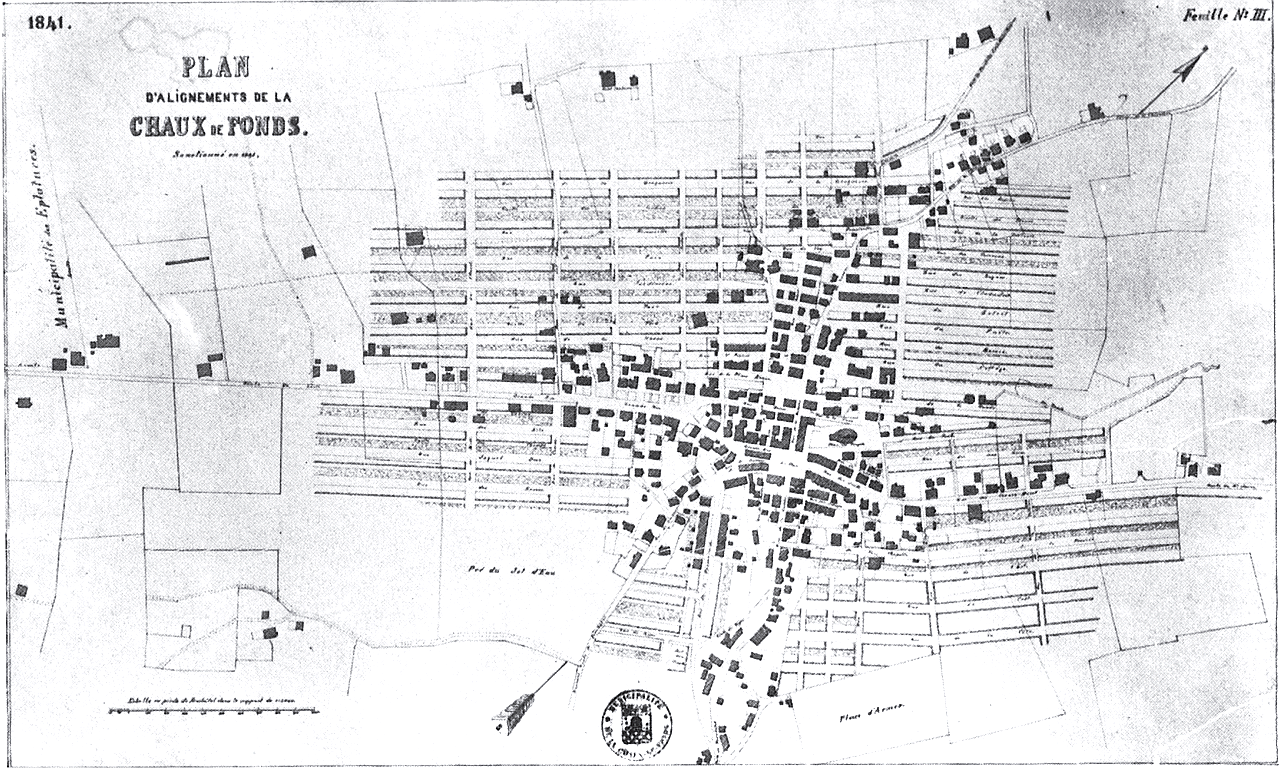
\includegraphics[width=\linewidth]{%
					images/la-chaux-de-fonds/1280px-La_Chaux-de-Fonds1841.png%
				}
				\caption{Development plan of La Chaux-de-Fonds from 1841\cite{Wikimedia:LaChauxDeFonds1841}}
				\label{fig:map:plan-la-chaux-de-fonds-1841}
			\end{figure}
			
			
			The plan designed a grid layout with rectangular blocks of around 45m x 125m\ref{fig:img:la-chaux-de-fonds-block-layout-1900}, containing one row of buildings, bordering to the street on one side and containing open space or yards on the other side.
			
			\begin{figure}[H]
				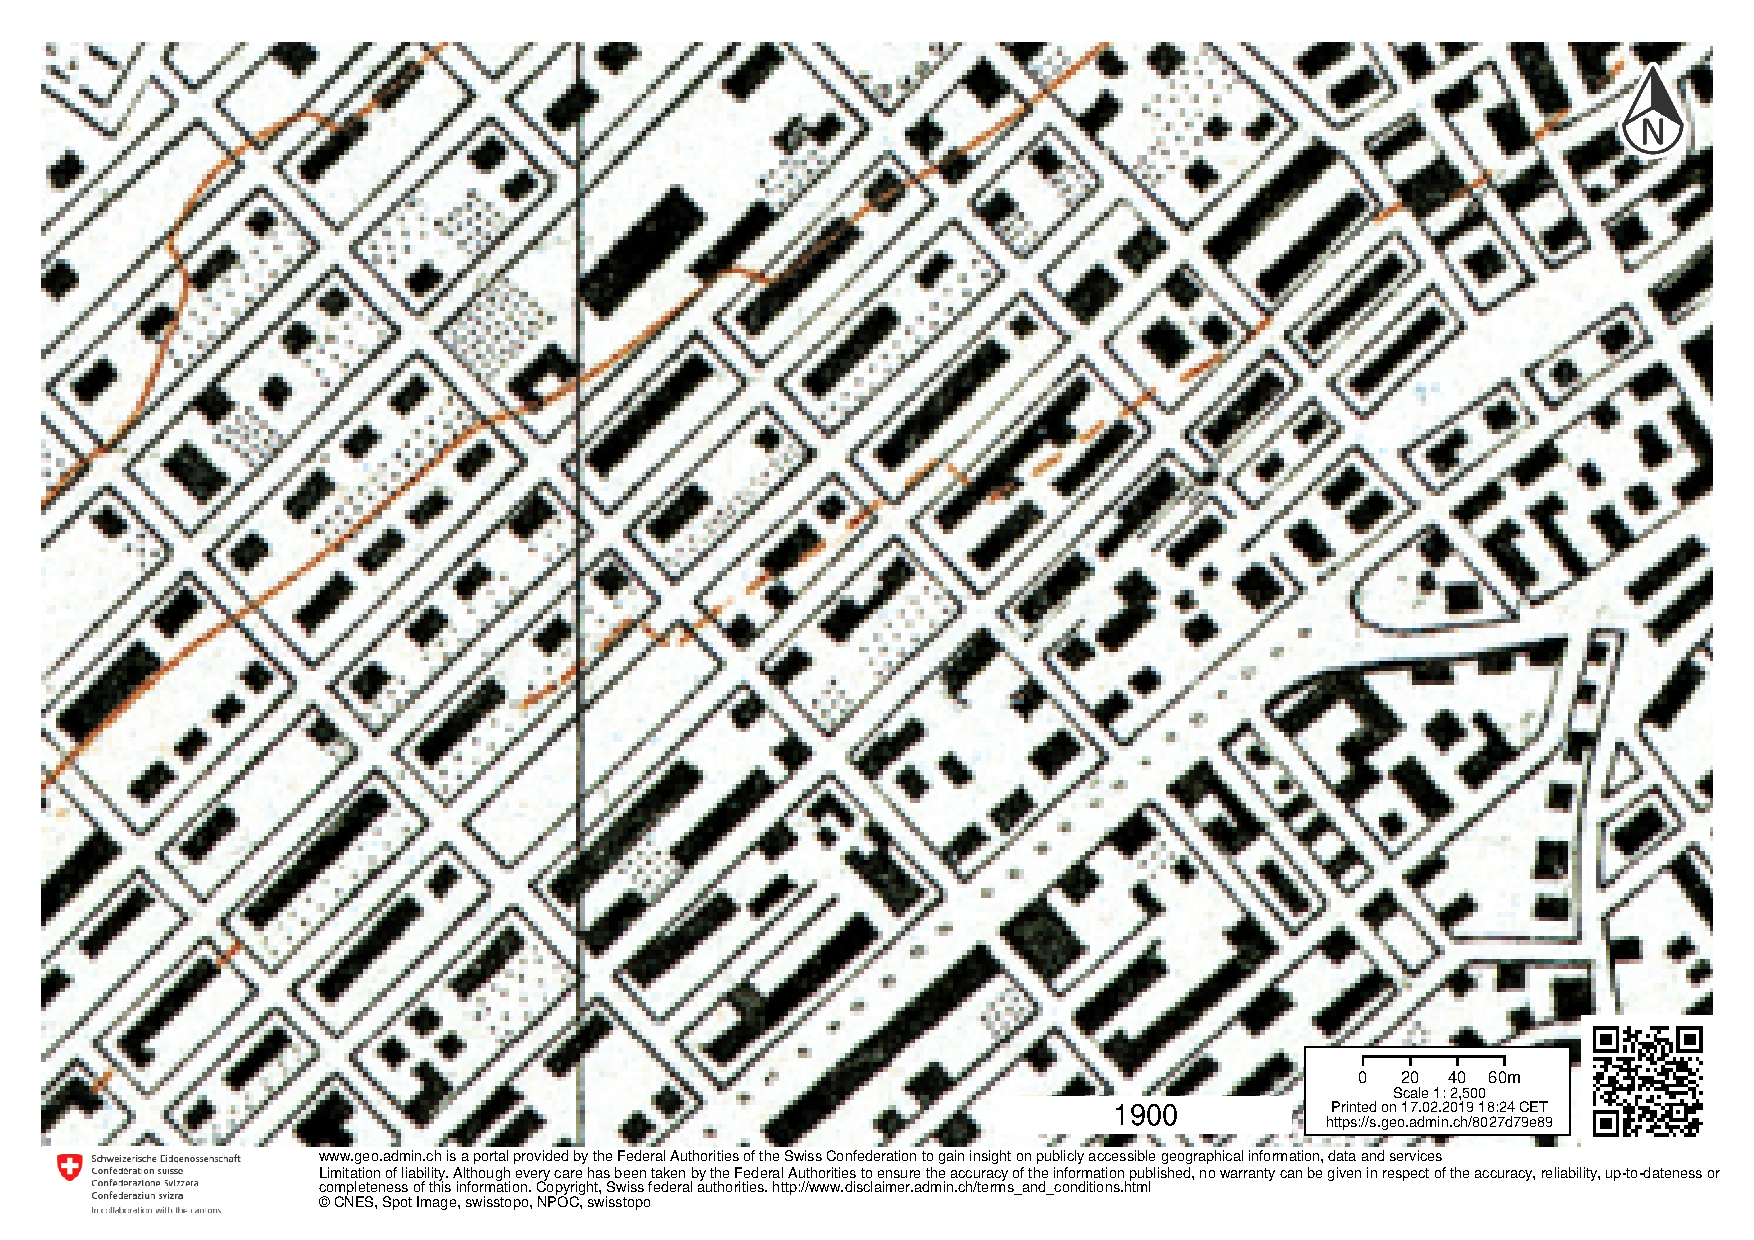
\includegraphics[width=\linewidth,trim={1cm 1cm 1cm 1cm}]{%
					images/la-chaux-de-fonds/block-layout-1900.pdf%
				}
				\caption{Block layout in La Chaux-de-Fonds 1900\cite{MapGeoAdmin:LaChauxDeFonds}. (The first map of that detail level of La Chaux-de-Fonds is available from 1897)}
				\label{fig:img:la-chaux-de-fonds-block-layout-1900}
			\end{figure}
			
			
			The city was planned for pedestrians, cyclists, horses and carts.
			It was planned as a compact city. Everything should be reachable by foot.
			
			
			\begin{figure}[H]
				\includegraphics[width=\linewidth,trim={1cm 1cm 1cm 1cm}]{%
					maps/la-chaux-de-fonds/1845.pdf%
				}
				\caption{La Chaux-de-Fonds 1945\cite{MapGeoAdmin:LaChauxDeFonds}}
				\label{fig:map:la-chaux-de-fonds-1945}
			\end{figure}
			
			Until 1870\ref{fig:map:la-chaux-de-fonds-1945}, there was not much development, the city kept their small size and only a few new blocks were developed.
			
			
			\subsubsection{Development}
			\begin{figure}[H]
				\includegraphics[width=\linewidth,trim={1cm 1cm 1cm 1cm}]{%
					maps/la-chaux-de-fonds/1900.pdf%
				}
				\caption{La Chaux-de-Fonds 1900\cite{MapGeoAdmin:LaChauxDeFonds}}
				\label{fig:map:la-chaux-de-fonds-1900}
			\end{figure}
			
			From 1870 to 1900\ref{fig:map:la-chaux-de-fonds-1900}, the city grew fast to a diameter of around 1.5kms, reaching the borders of the plan from 1841.
			1900 it was already connected by four national railway lines and streetcar lines were under construction.
			% TODO pictures from La Chaux de Fonds 1888
			% http://cdf-bibliotheques.ne.ch/bvcf/patrimoine/dossiers-thematiques/plans/Pages/reconstruction_a_1888.aspx
			
			
			\begin{figure}[H]
				\includegraphics[width=\linewidth,trim={1cm 1cm 1cm 1cm}]{%
					maps/la-chaux-de-fonds/1960.pdf%
				}
				\caption{La Chaux-de-Fonds 1960\cite{MapGeoAdmin:LaChauxDeFonds}}
				\label{fig:map:la-chaux-de-fonds-1960}
			\end{figure}
			% TODO put map from 1954 (first sprawled districts)
			
			From 1900 to 1950\ref{fig:map:la-chaux-de-fonds-1960}, the city continued growing fast, continuing the pattern the plan from 1841 had defined. The city reached a diameter of around 2kms. 
			Also the development reached the station and continued on the other side, but kept growing only at the base of the valley.
			The city still was compact, pedestrian, cyclist and streetcar oriented.
			
			
			\begin{figure}[H]
				\includegraphics[width=\linewidth,trim={1cm 1cm 1cm 1cm}]{%
					images/la-chaux-de-fonds/sprawling-development-1960.pdf%
				}
				\caption{Sprawling development in La Chaux-de-Fonds around 1960\cite{MapGeoAdmin:LaChauxDeFonds}}
				\label{fig:map:la-chaux-de-fonds-sprawling-development-1960}
			\end{figure}
			
			From 1950\ref{fig:map:la-chaux-de-fonds-sprawling-development-1960} the development started crawling up the hills around La Chaux-de-Fonds.
			New districts with big yards and lower density were constructed fast.
			The development did not follow anymore the planned pattern from 1841.
			
			
			Because of the growing popularity of the automobile, the street network was intensively extended and streets were paved.
			Also industrial parks in the outlying areas were constructed.
			
			Since 1980 Switzerland counts with land-use planning laws and zone planning. Zone planning restricts development outside of development zones. Anyhow increased the development area in Switzerland since 1950 by 100\%.
			The restrictive zone planning slowed the sprawling development in La Chaux-de-Fonds down.
			
			
			\subsubsection{Today}
			
			Today\ref{fig:map:la-chaux-de-fonds-2018}, La Chaux-de-Fonds is around 5kms long and 2.5km wide. Several districts at the hillside provide expensive apartments and houses to solvent inhabitants.
			% TODO Picture of hillside constructions
			
			\begin{figure}[H]
				\includegraphics[width=\linewidth,trim={1cm 1cm 1cm 1cm}]{%
					maps/la-chaux-de-fonds/2018.pdf%
				}
				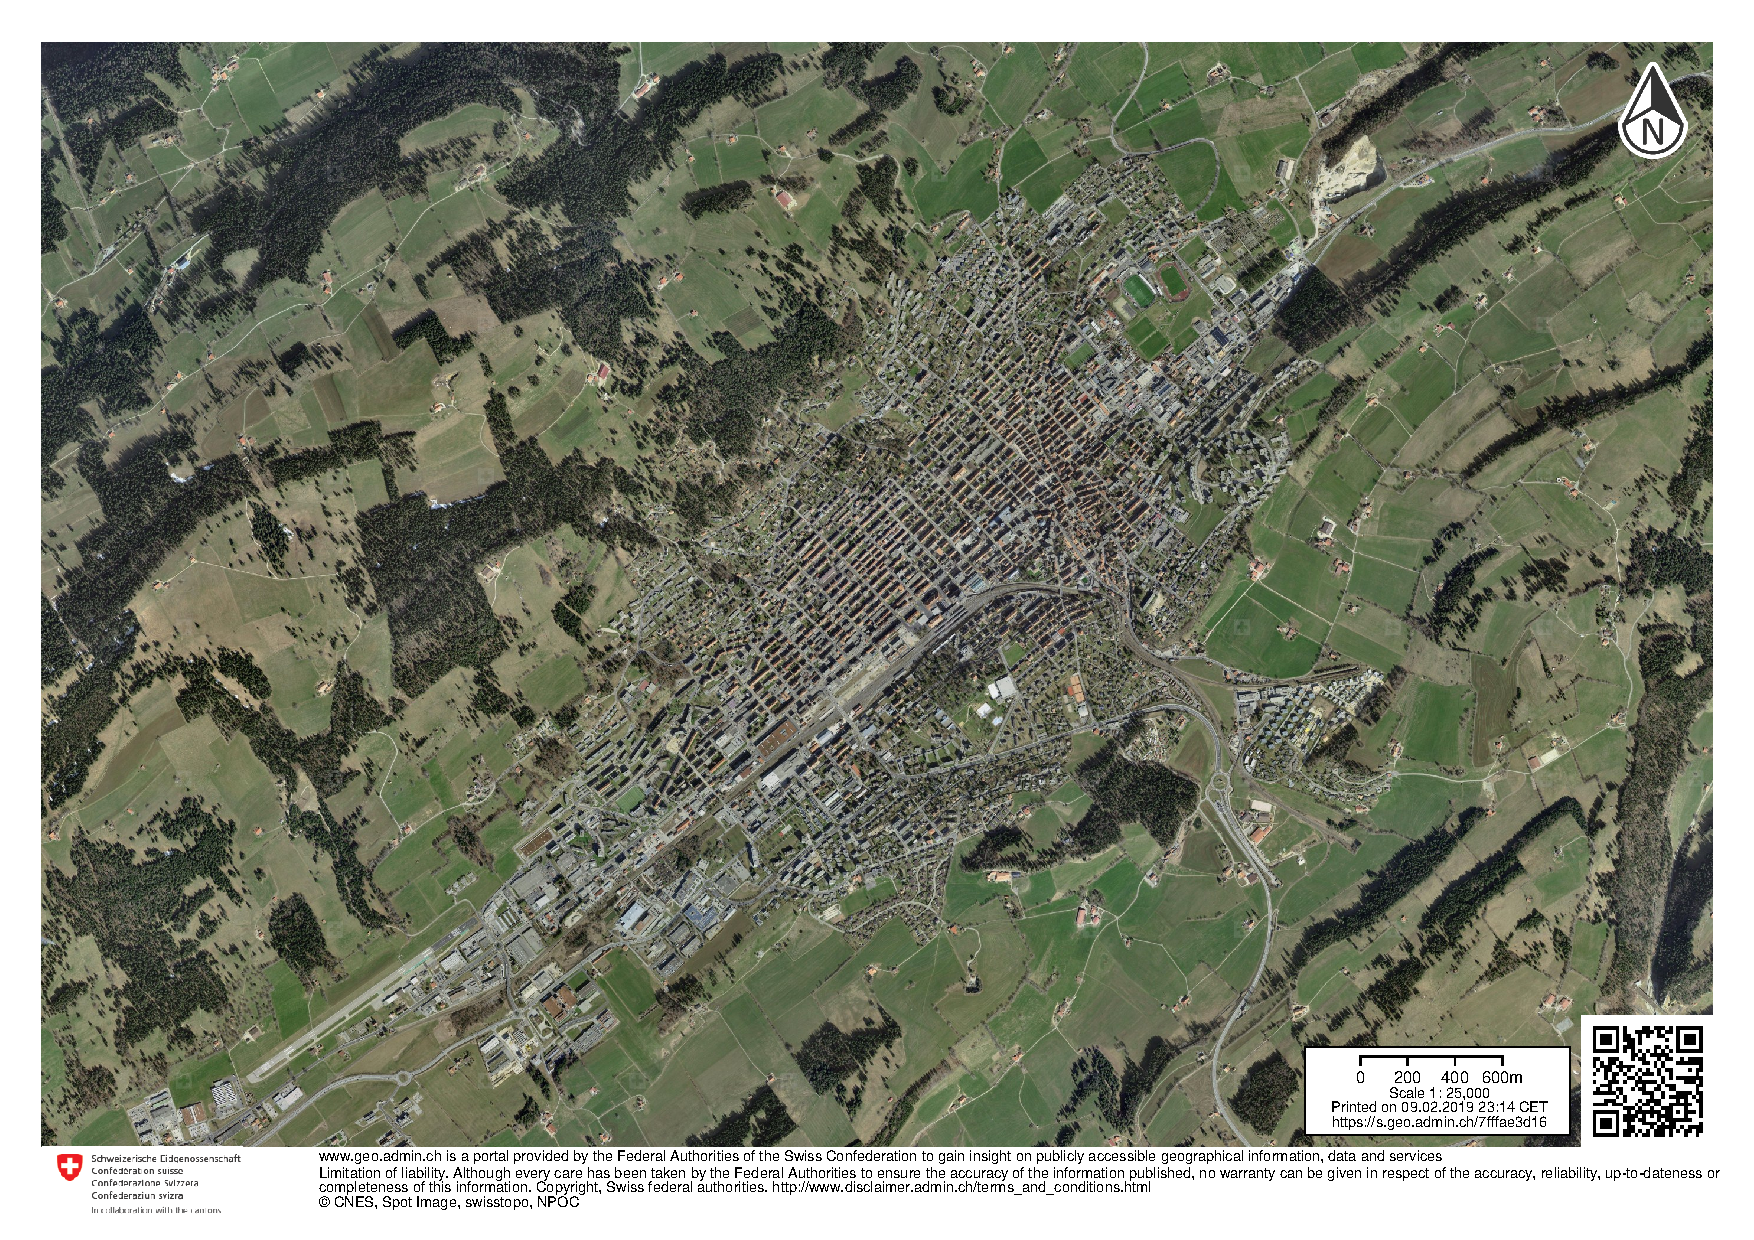
\includegraphics[width=\linewidth,trim={1cm 1cm 1cm 1cm}]{%
					images/la-chaux-de-fonds/areal-2019.pdf%
				}
				\caption{La Chaux-de-Fonds 2018\cite{MapGeoAdmin:LaChauxDeFonds}}
				\label{fig:map:la-chaux-de-fonds-2018}
			\end{figure}
			
			Because of it's general high density, La Chaux-de-Fonds counts with good transit\ref{fig:la-chaux-de-fonds-public-transport} options. Even if the streetcar lines do not exist anymore, an extensive bus network reaches also districts up in the hills.
			
			
			% TODO Haltestellen karte map geo admin
			
			\begin{figure}[H]
				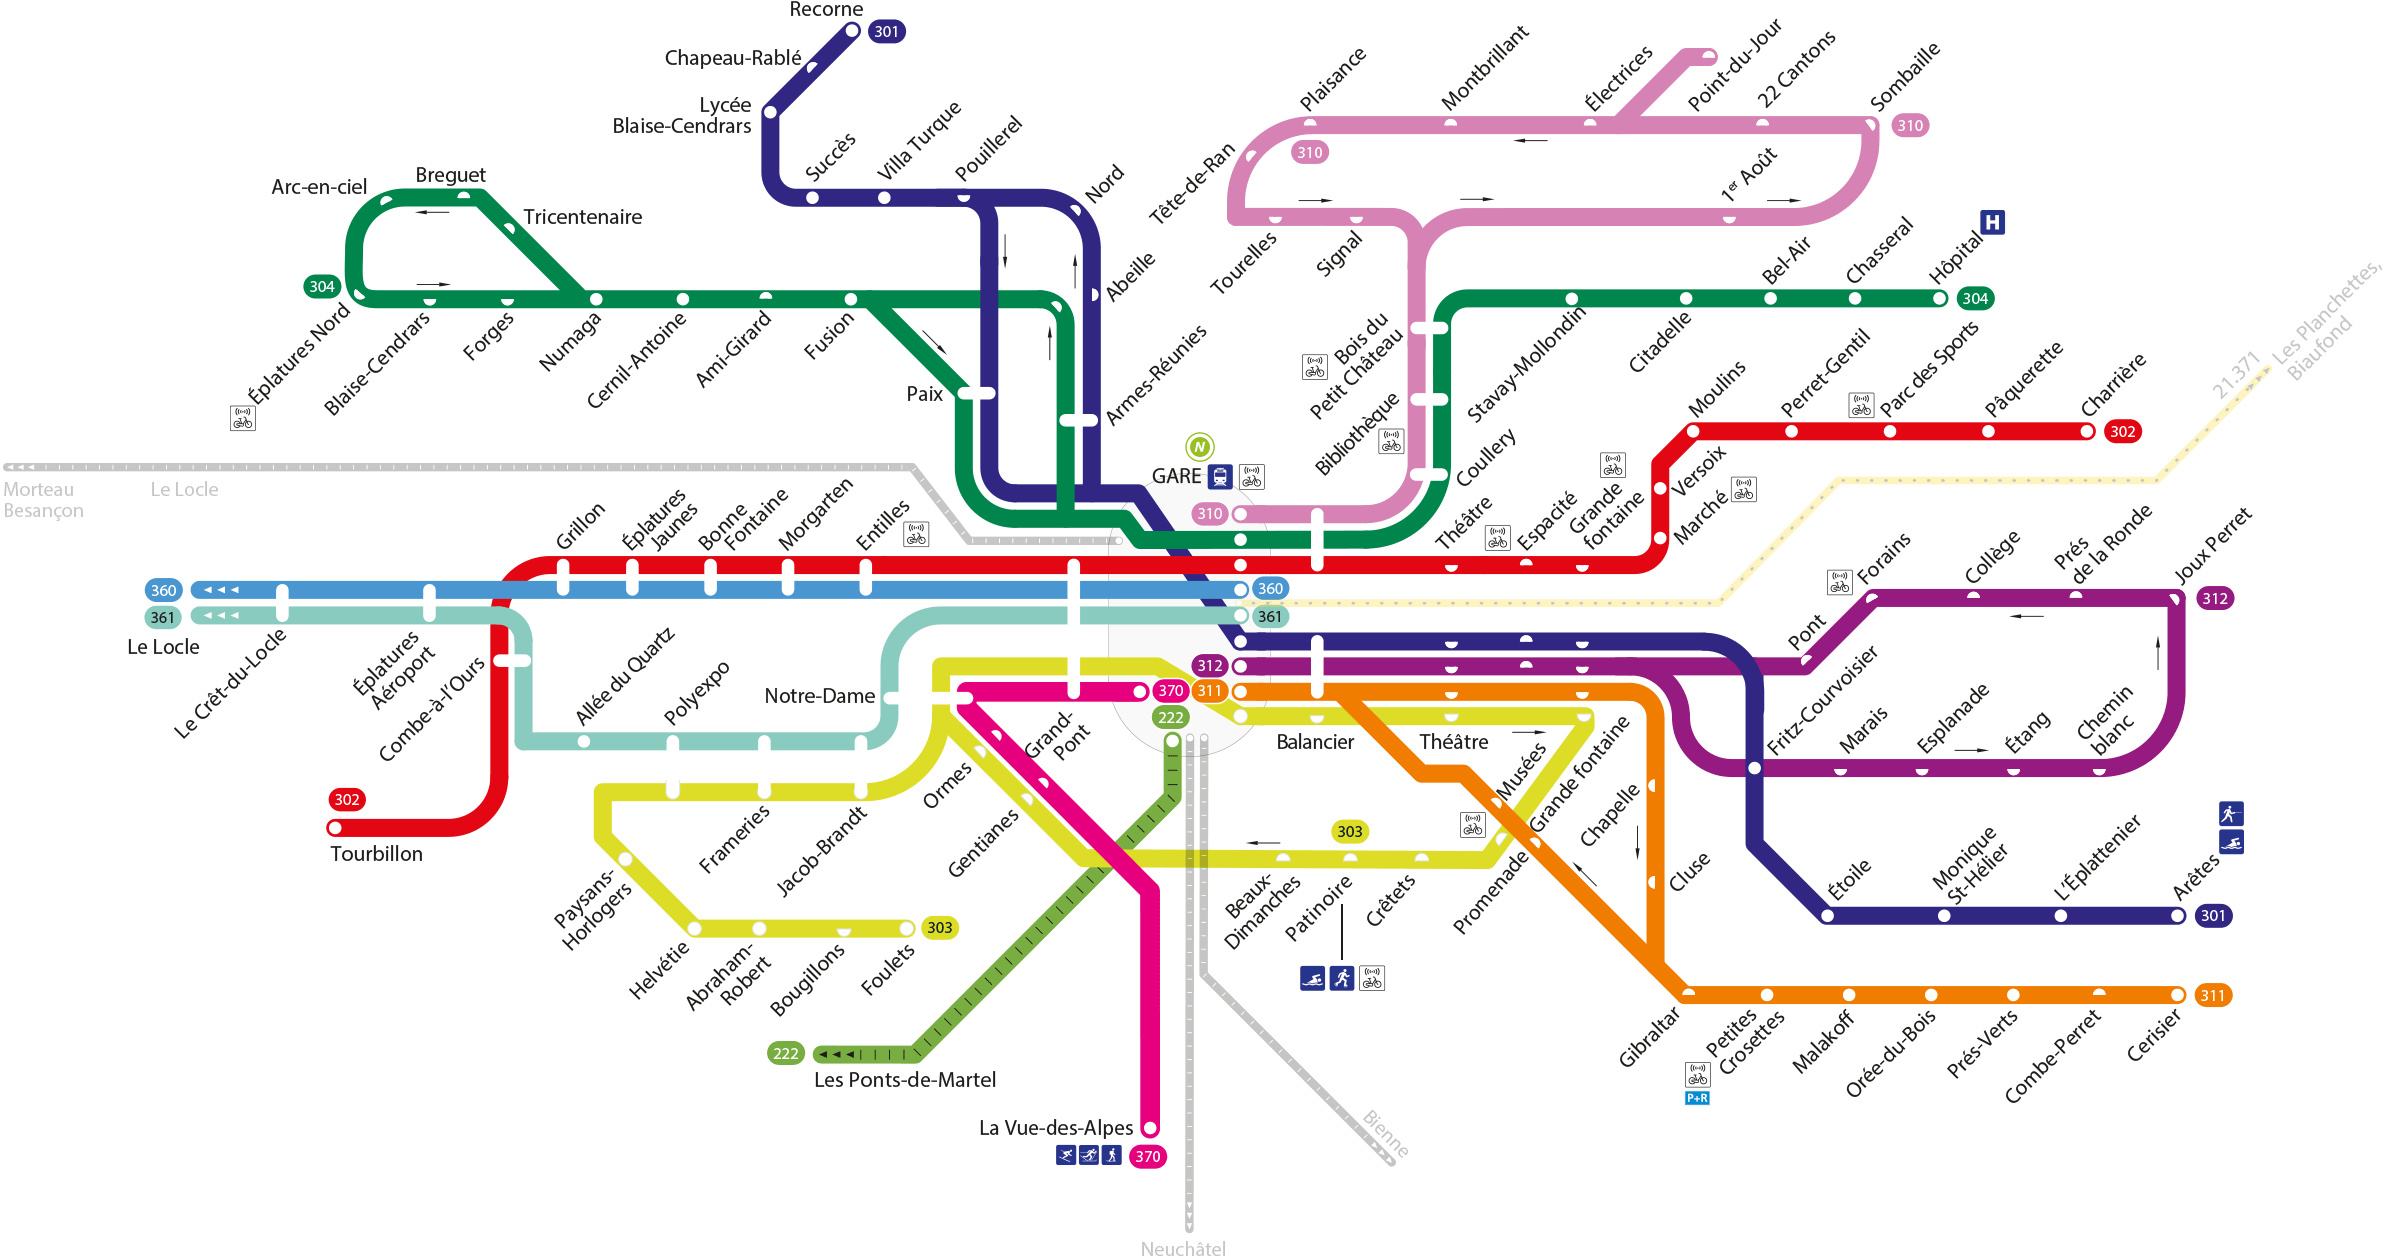
\includegraphics[width=\linewidth]{%
					images/la-chaux-de-fonds/public-transport-plan.jpg%
				}
				\caption{La Chaux-de-Fonds public transport network\cite{TransN:LaChauxDeFonds}}
				\label{fig:la-chaux-de-fonds-public-transport}
			\end{figure}
			
			
			\subsubsection{Roundup}
			% TODO growth ring map
			La Chaux-de-Fonds was planned as a pedestrian city in it's time.
			The arrival of the automobile caused the construction of low density districts.
			But the geographical location in the valley and the zone restrictions since 1980 limited the city from sprawling out.
			La Chaux-de-Fonds ist still a pedestrian friendly and compact city and counts with great public transport services.
			
			
		\clearpage
		\begin{strip}
		\subsection{La Plata, Argentina}
		\end{strip}
		
			% TODO La Plata world map
			
			\subsubsection{Original Plan}
			Buenos Aires, the biggest and most powerful city of Argentina, was national and state capital. To reduce the power and separate political interests, a new capital for the state Buenos Aires was planned and funded in 1882.
			The city was located 10kms inland of the river coast at the railway line from Ensenada to Buenos Aires, around 50kms away from the capital.
			
			\begin{figure}[H]
				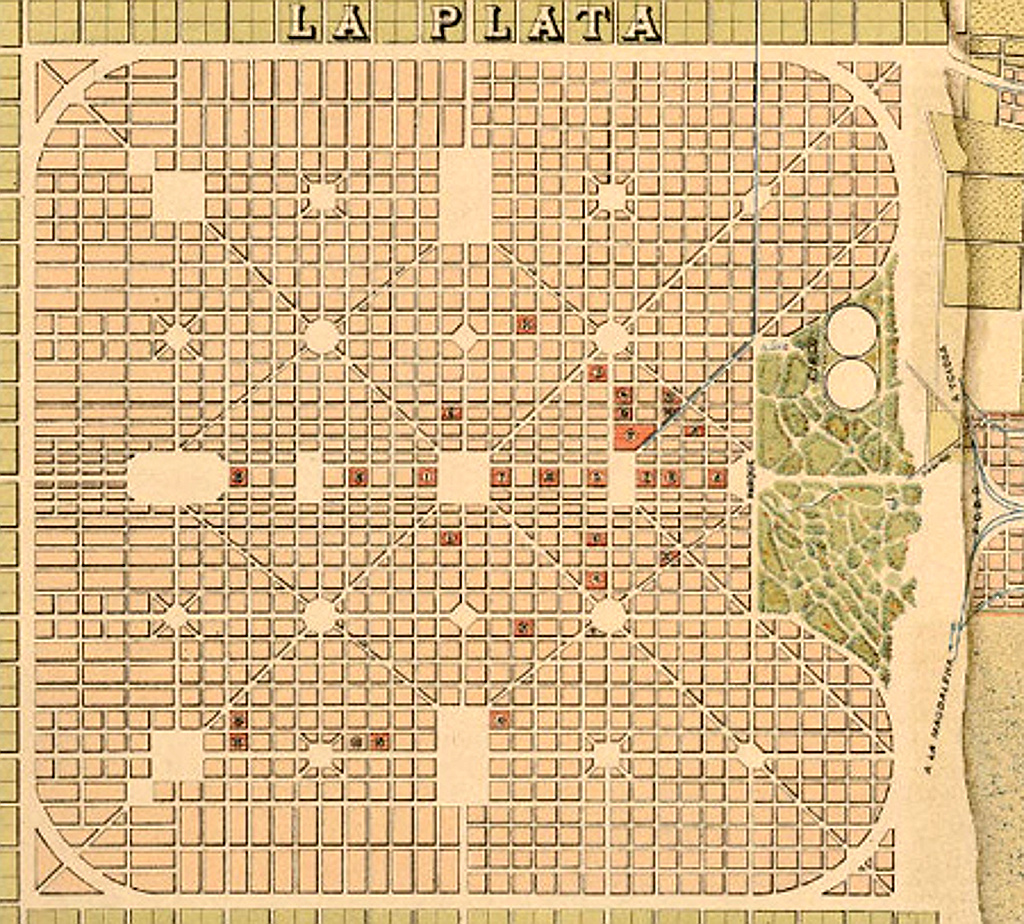
\includegraphics[width=\linewidth]{%
					images/la-plata/planolaplata.jpg%
				}
				\caption{La Plata grid plan, designed by Pedro Benoit, 1882\cite{RecoletaCemetery:PedroBenoit}}
				\label{fig:img:plan-la-plata-1882}
			\end{figure}
			
			The plan shows a 38 x 38 block grid, criss-crossed by diagonals and most of the city’s government buildings and major churches.
			
			The diagonal boulevards are have been preserved and are a characteristic of La Plata until today.
			
			Many suburbs were founded together with the city:
			- Los Hornos
			- Ringuelet
			- San Carlos
			
			
			Some existed before and were merged, when the city was founded:
			- Tolosa
			- Altos de San Lorenzo
			
			% https://es.wikipedia.org/wiki/Gran_La_Plata
			
			
			\subsubsection{Development}
			
			
			\begin{figure}[H]
				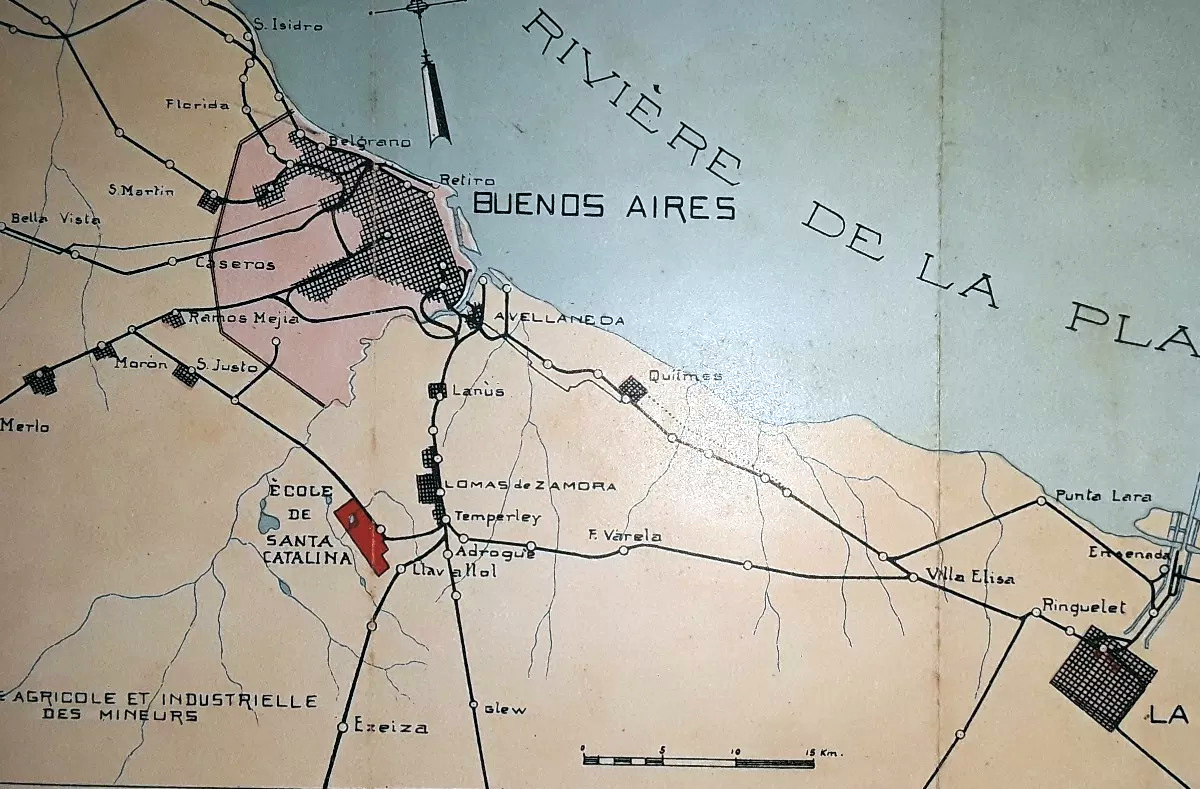
\includegraphics[width=\linewidth]{%
					maps/la-plata/1901-buenosaires-laplata.jpg%
				}
				\caption{Buenos Aires and La Plata 1901\cite{RiviereDeLaPlata}}
				\label{fig:map:buenosaires-la-plata-1901}
			\end{figure}
			% https://http2.mlstatic.com/plano-1901-buenos-aires-la-plata-D_NQ_NP_615971-MLA28714158588_112018-F.webp
			
			
			% TODO Images from La Plata from 1900
			% La Plata 1885 http://construirtv.com/wp-content/uploads/2015/10/ciudad-mirando-al-oeste_Bradley.jpg
			
			In the first 20 years, the city grew fast, government buildings were constructed, streetcar lines were opened, the university was founded.
			
			% 1932 Palacio Municipal
			% https://es.wikipedia.org/wiki/Archivo:Palacio_Municipal_y_Eje_Fundacional_de_La_Plata_(1932).jpg
			
			% Historic fotos of la plata
			% https://www.taringa.net/+imagenes/historia-y-fotos-de-la-catedral-de-la-plata_z48jx
			
			% http://www.gotakey.com/blog/14/04/2016/porque-la-plata-tiene-tantas-diagonales/
			
			
			
			\begin{figure}[H]
				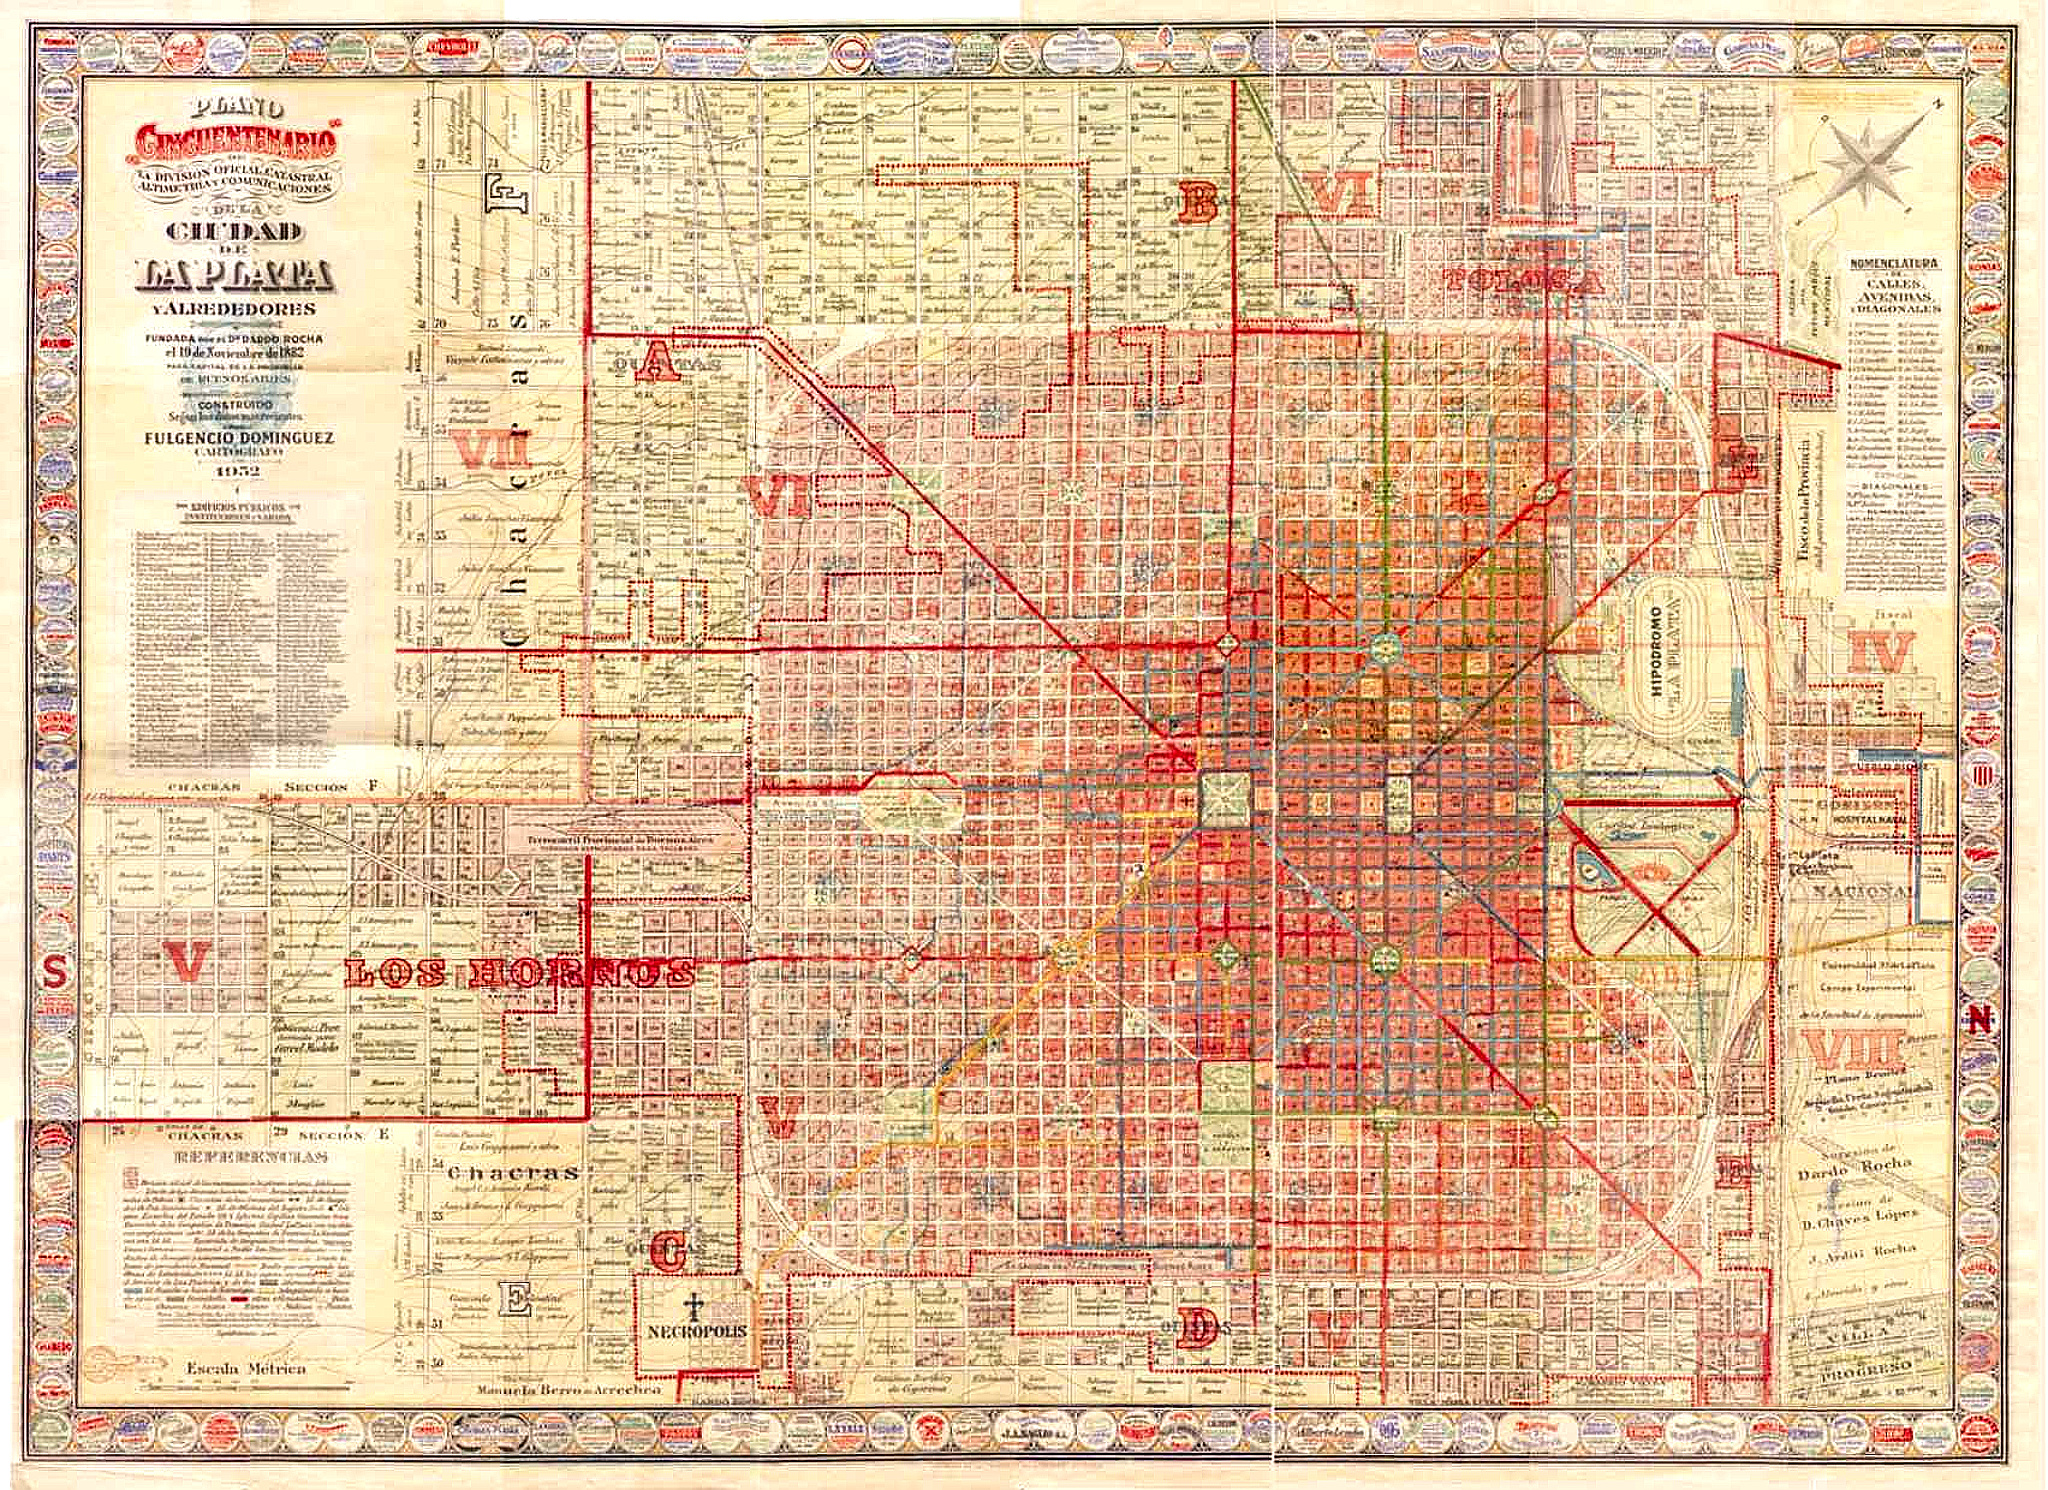
\includegraphics[width=\linewidth,trim={1.5cm 1.5cm 1.5cm 1.5cm},clip]{%
					images/la-plata/la_plata_1952.jpg%
				}
				\caption{La Plata 1952\cite{MOSP:InvestigacionHistorica}}
				\label{fig:map:la-plata-1952}
			\end{figure}
			
			\begin{figure}[H]
				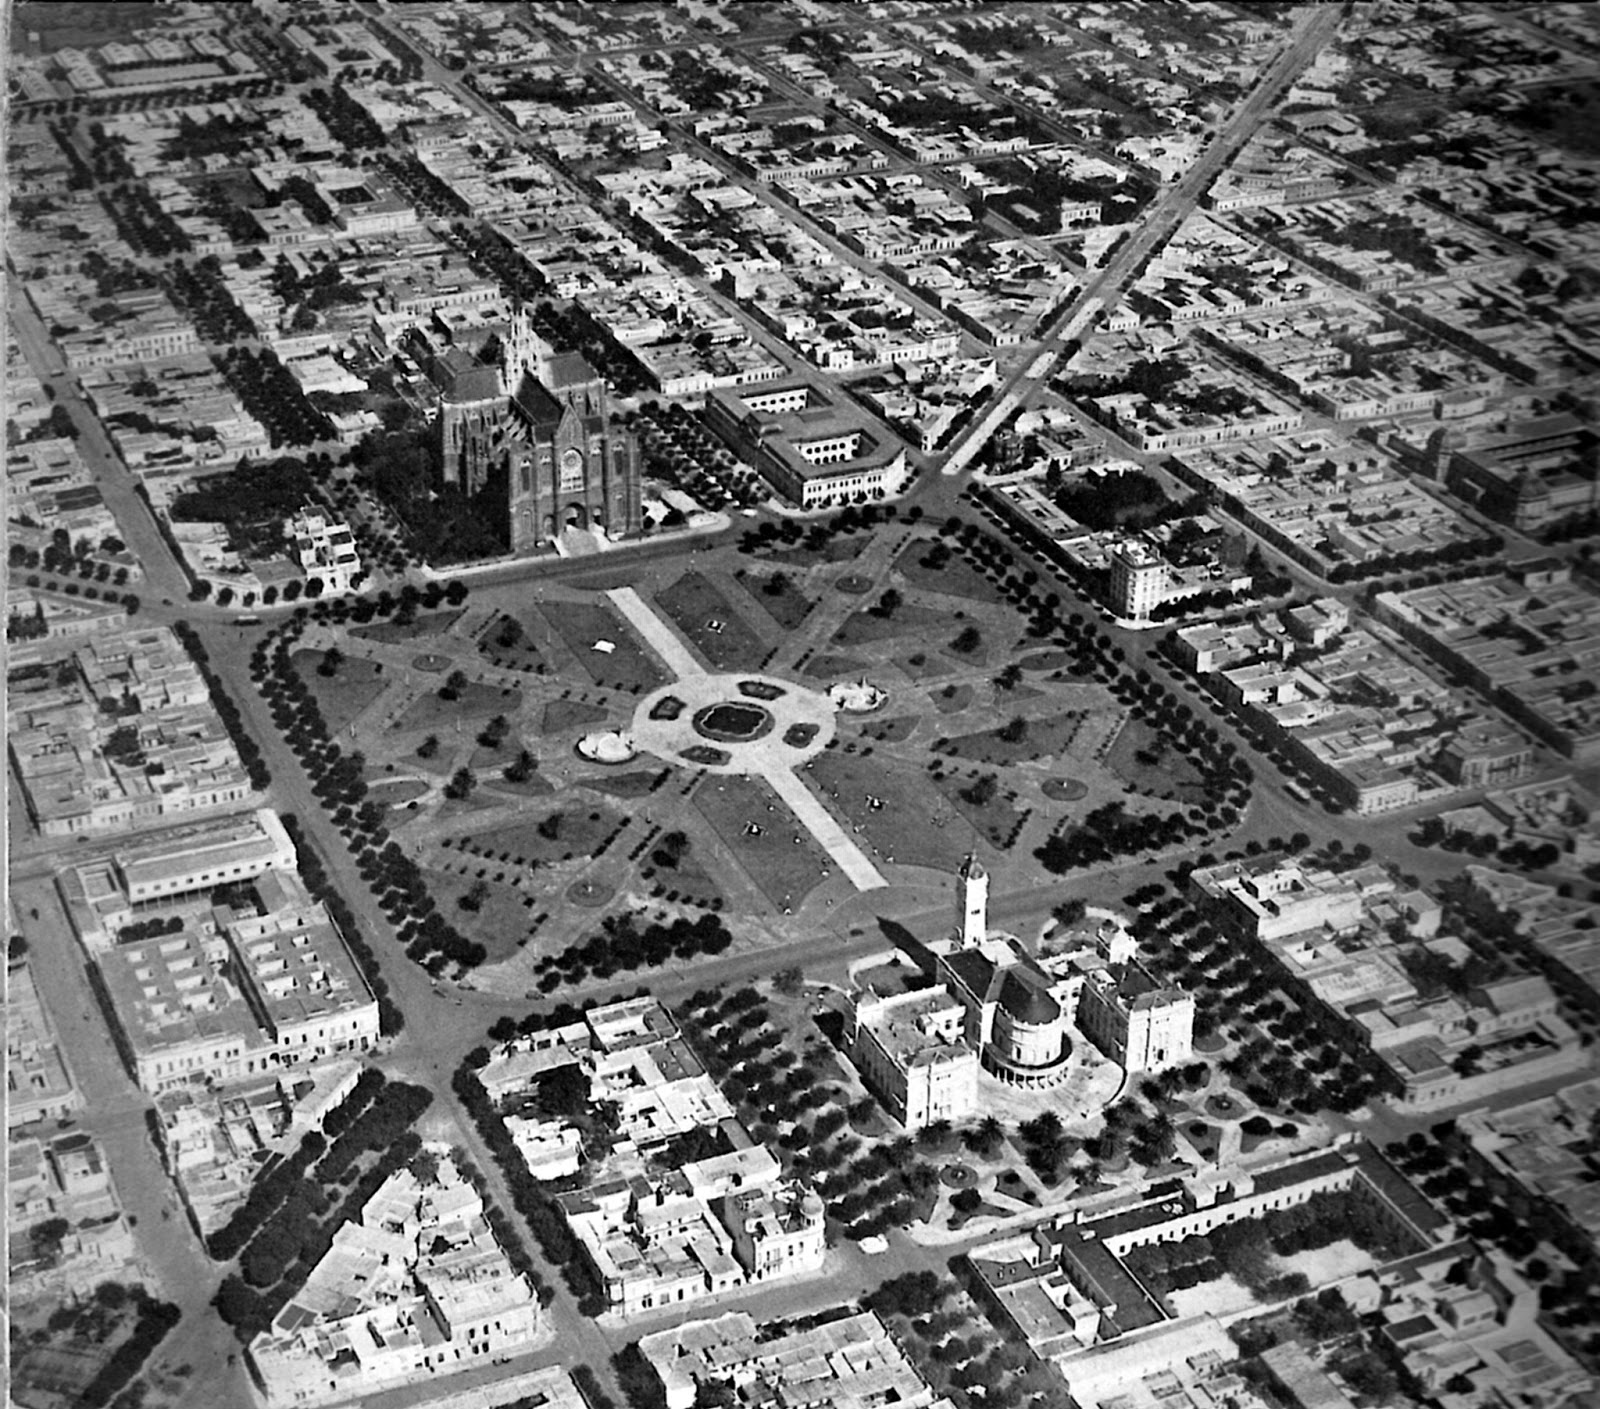
\includegraphics[width=\linewidth]{%
					images/la-plata/plaza-central-1940.jpg%
				}
				\caption{Plaza Mariano Moreno of La Plata 1940\cite{Blogspot:Arqruotolo:la-plata-o-la-geometria-hecha-espacio}}
				\label{fig:img:la-plata-1940}
			\end{figure}
			1952: In Tolosa, Los Hornos and Villa Elvira, the city already grew outside of the layout from 1882.
			
			1950: Around 300'000 inhabitants.
			The city is bursting out of its design pattern. 
			
			% http://bibliotecadigital.uns.edu.ar/scielo.php?script=sci_arttext&pid=S1852-42652013001100002&lng=es
			% http://bibliotecadigital.uns.edu.ar/pdf/reuge/v22n1/v22n1a02.pdf
			
			
			
			2000: More than 650'000 inhabitants.
			
			\begin{center}
	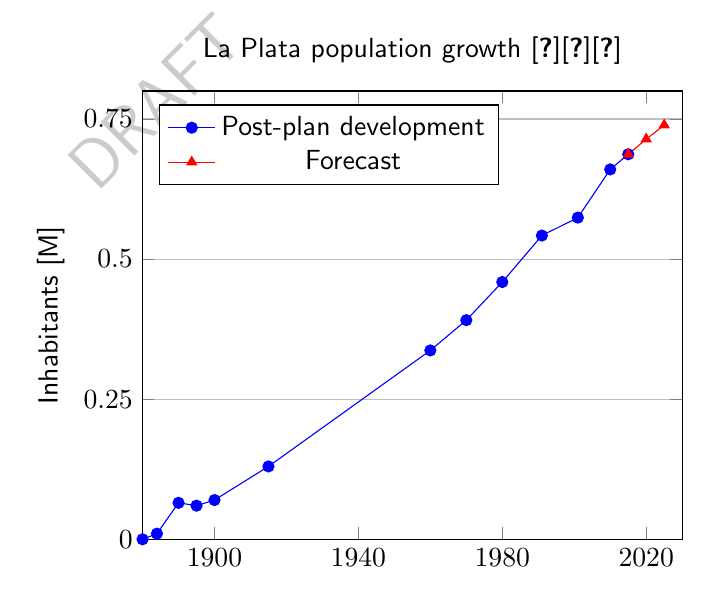
\begin{tikzpicture}[>=latex]
		\begin{axis}[
				title={La Plata population growth \cite{CityPopulation:LaPlata}\cite{Wikipeda:LaPlataHistory}\cite{ElDiaSa:LaPlata2025}},
				style={/pgf/number format/1000 sep=},
				ylabel={Inhabitants [M]},
				xmin=1880, xmax=2030,
				ymin=0, ymax=0.8,
				xtick={1900,1940,1980,2020},
				ytick={0,0.25,0.5,0.75},
				legend pos=north west,
				ymajorgrids=true
			]				
			\addplot[color=blue,mark=otimes*] coordinates {
				(1880,0)(1884,0.01)(1890,0.065)(1895,0.06)(1900,0.07)(1915,0.13)(1960,0.337)(1970,0.391)(1980,0.459)(1991,0.542)(2001,0.574)(2010,0.660)(2015,0.687)
			};
			\addplot[color=red,mark=triangle*] coordinates {
				(2015,0.687)(2020,0.714)(2025,0.739)
			};
			
			\legend{Post-plan development, Forecast}				
		\end{axis}
	\end{tikzpicture}	
\end{center}

		
			
			
			\subsubsection{Today}
			
			\begin{table}[H]			
				\centering
				\caption{Facts}
				\label{table:la-plata-facts}
				\begin{tabular}{|l|l|}
					\hline
					\textbf{Population (2015)} & \textgreater 0.8 M \\
					\textbf{Density}           & ~40 pop./ha \\
					\hline
				\end{tabular}
			\end{table}
			
			Today La Plata has around 700'000 inhabitants. The city spreads over an aeria\ref{fig:map:la-plata-2019} which has multiple times the size of the original plan from 1882.			
			
			\begin{figure}[H]
				\includegraphics[width=\linewidth]{%
					maps/la-plata/2019.jpg%
				}
				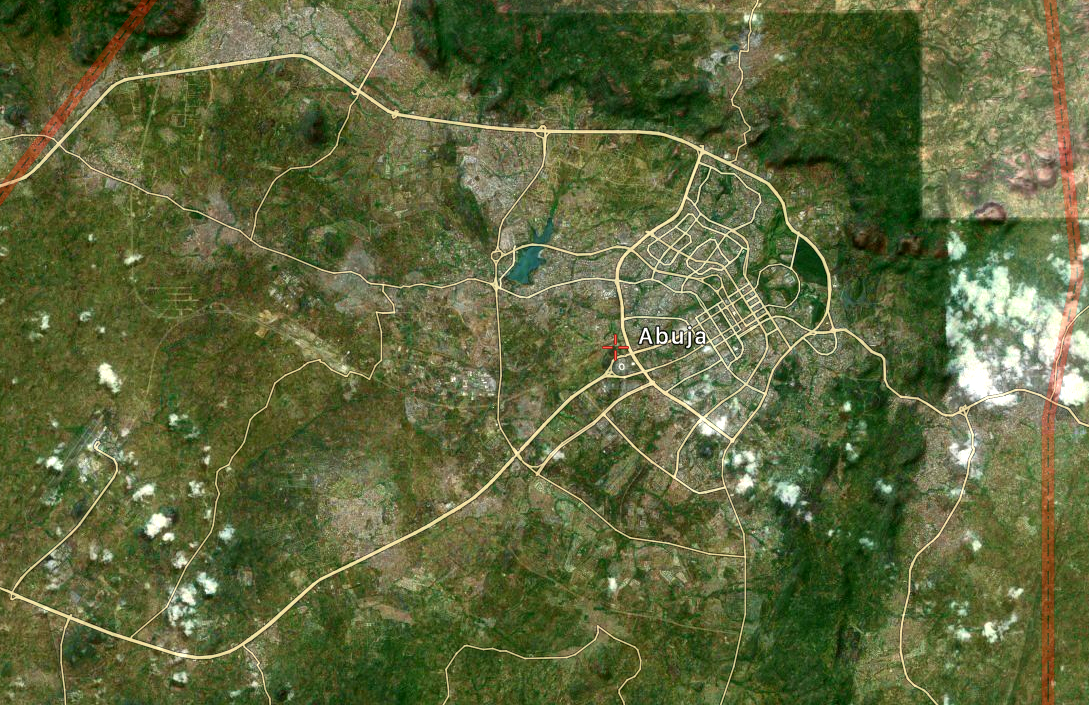
\includegraphics[width=\linewidth]{%
					images/la-plata/2019-aerial.jpg%
				}
				\caption{La Plata 2019\cite{OpenStreetMap:LaPlata}}
				\label{fig:map:la-plata-2019}
			\end{figure}
			
			The last streetcar line was closed down in 1966, today La Plata counts with 23 bus lines\ref{fig:map:la-plata-transit} connecting the city center and the suburbs.
			The outer suburbs are not well connected by public transit and mostly car-dependent.
			
			\begin{figure}[H]
				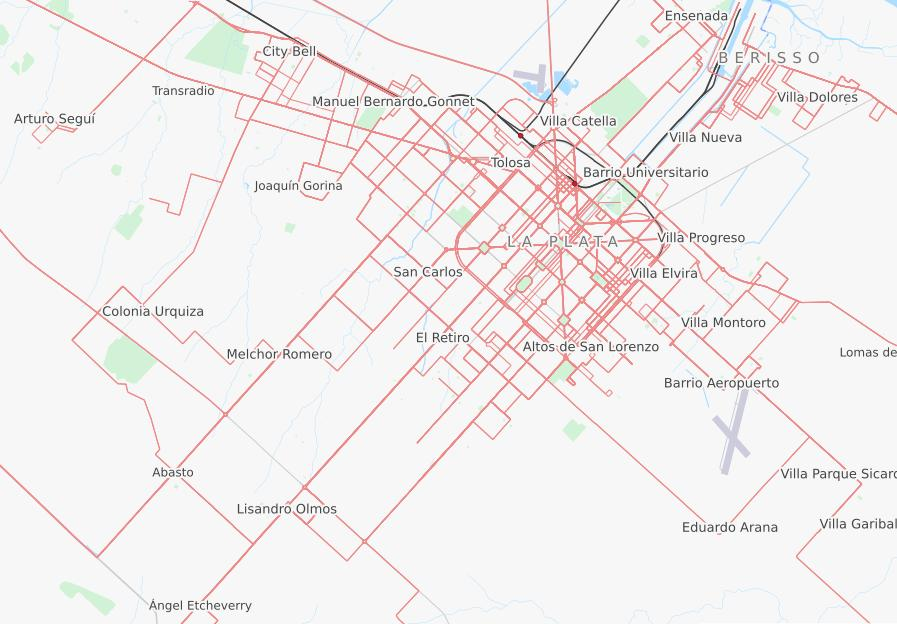
\includegraphics[width=\linewidth]{%
					maps/la-plata/transit-lines.jpg%
				}
				\caption{La Plata public transportation\cite{OpenStreetMap:LaPlata}}
				\label{fig:map:la-plata-transit}
			\end{figure}
			
			% TODO cycle map
			
			
			\subsubsection{Roundup}
			
			
			
		\clearpage
		\begin{strip}
		\subsection{Abuja, Nigeria}
		\end{strip}
		
			% TODO Abuja world map
			
			% http://www.newtowninstitute.org/spip.php?article1050
			
			\subsubsection{Original Plan}
			
			Abuja was planned 1976, to replace Lagos as former capital.
			The new capital should resolve the problems of the population growth concentration in Lagos, and also represent better the ethnics from the different parts of the country.
			
			The new capital was planned in the middle of the country, being reachable by similar travel distances from all regions, but far away from existing rail way lines and highways.
			
			\begin{figure}[H]
				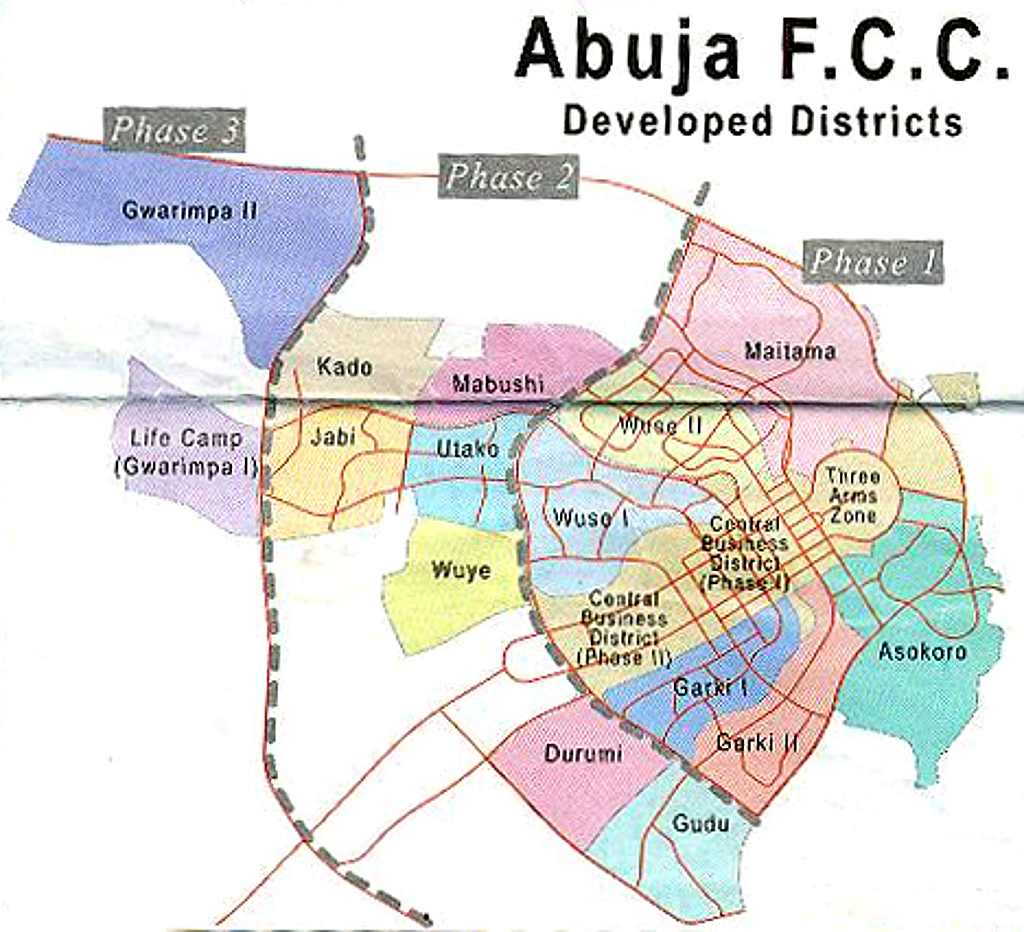
\includegraphics[width=\linewidth]{%
					maps/abuja/abuja-development-map.jpg%
				}
				\caption{Abuja development plan\cite{NairalandForum:AbujaMap}}
				\label{fig:map:abuja-development-plan}
			\end{figure}
			
			Abuja's master plan was developed by 3 American firms and the central business district was designed by a Japanese architect.
			
			The layout of the city was car oriented designed. Districts count with small commercial zones but the most of the commercial and business activity is located in the Central Business District.
			
			\begin{figure}[H]
				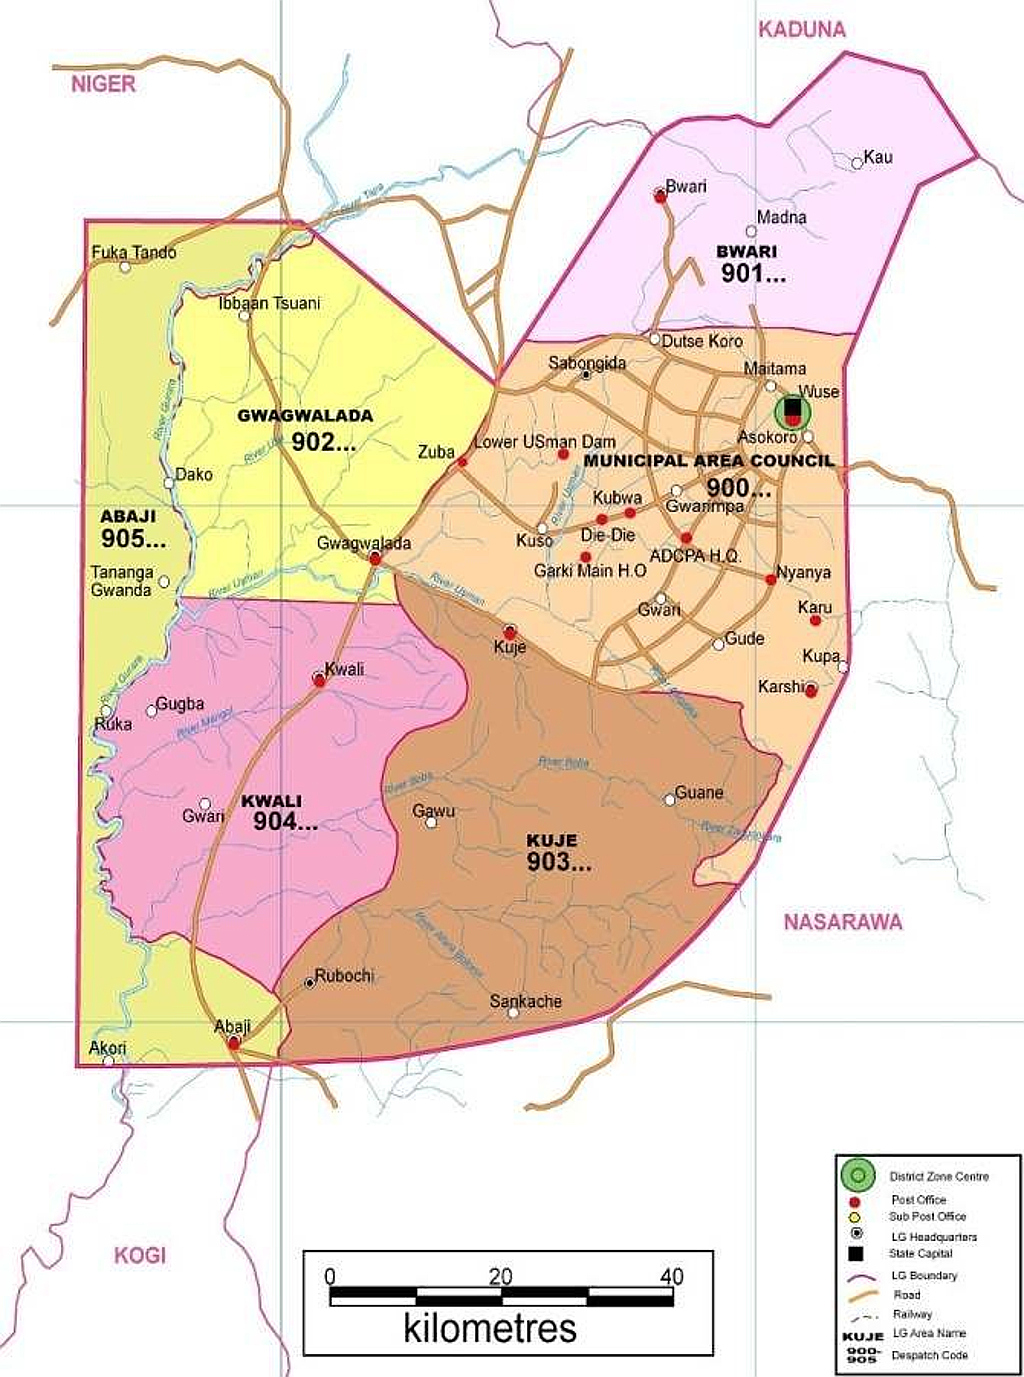
\includegraphics[width=\linewidth]{%
					maps/abuja/abuja-councils-map.jpg%
				}
				\caption{Six area councils of Abuja\cite{ResearchGate:SixCouncils}}
				\label{fig:map:abuja-six-area-councils}
			\end{figure}
			
			Residential districts were designed as closed networks in a cul-de-sac like style and do not allow to walk or drive directly to the next district. The districts itself count partially with grid-layouts, but to leave the district, there are often only one ore to entrance roads.
			
			In the Central Business District, 200m blocks were planned with pedestrian friendly infrastructure.
			The arterials were planned with level-free crossings for high traffic capacity.
			
			\begin{figure}[H]
				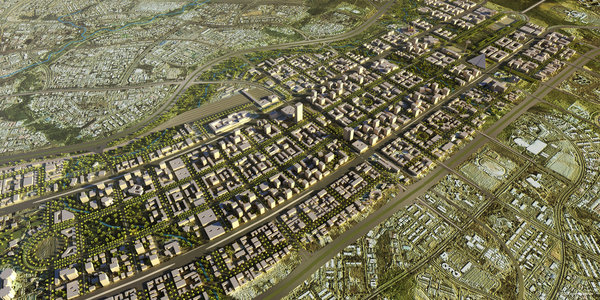
\includegraphics[width=\linewidth]{%
					images/abuja/csm_image1_2929afe067.jpg%
				}
				\caption{Master Plan for the central business district of Abuja\cite{ASplusP:MasterPlanReview}}
				\label{fig:map:abuja-master-plan-cbd}
			\end{figure}	
			
			It was planned to connect Abuja to the new national railway network, which should interconnect Nigeria from north to south and from east to west.
			Railway links were planned to Kaduna, Minna and Lafina.
			
			Eight metropolitan railway and light rail lines were planned, to connect the different districts and councils. 
			
			\begin{figure}[H]
				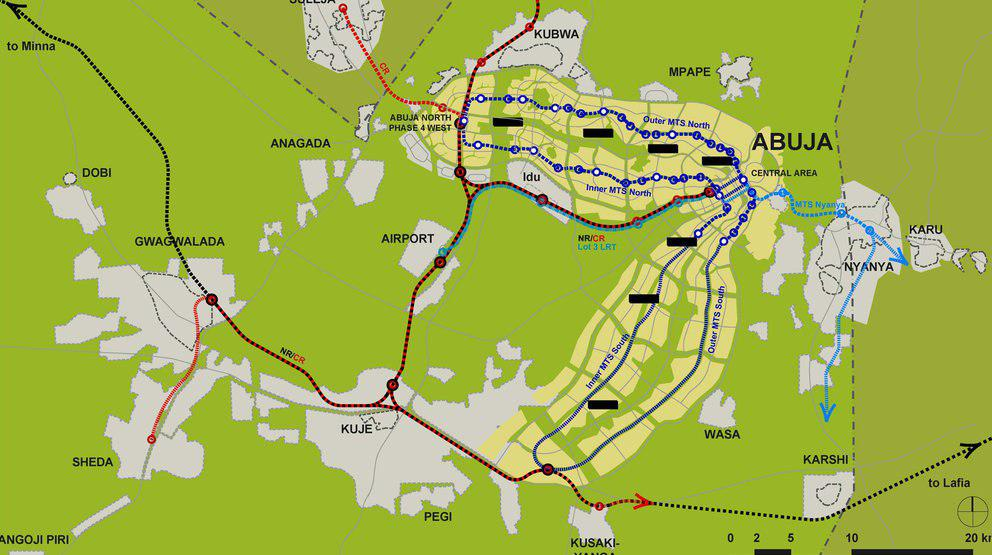
\includegraphics[width=\linewidth]{%
					maps/abuja/public-transport.jpg%
				}
				\caption{Abuja future rail transport network\cite{ASplusP:AbujaTransportationConcept}}
				\label{fig:map:abuja-future-rail-network}
			\end{figure}	
			
			
			\subsubsection{Development}
			
			The construction of the city started by constructing the Central Business District and the first highway ring, the initial stages were completed around 1980.
			
			15 years after its foundation, Abuja was officially declared as the capital. International companies and organizations moved their offices to Abuja.
			The development of the city increased, meanwhile the construction of public infrastructure continued slowly. Organizational problems and corruption hindered many projects.
			
			Many slums started to develop fast, spreading out of the originally planned area.

			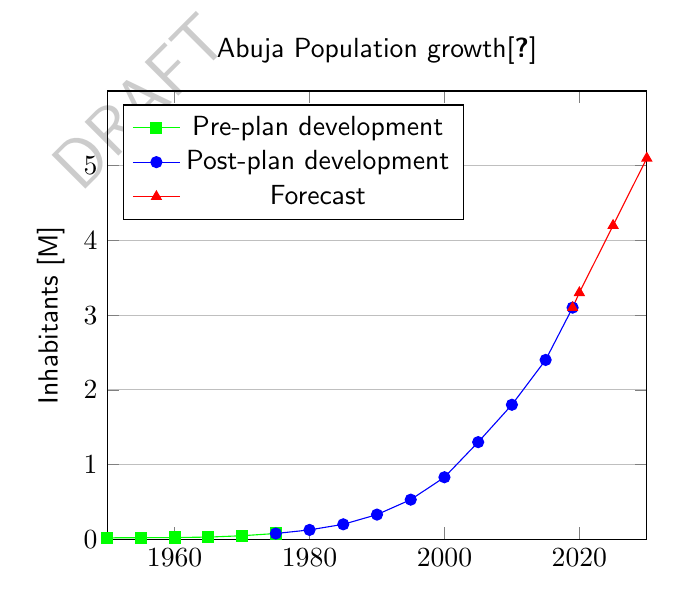
\begin{tikzpicture}[>=latex]
	\begin{axis}[
			title={Abuja Population growth\cite{WorldPopulationReview:Abuja}},
			style={/pgf/number format/1000 sep=},
			ylabel={Inhabitants [M]},
			xmin=1950, xmax=2030,
			ymin=0, ymax=6,
			xtick={1960,1980,2000,2020},
			ytick={0,1,2,3,4,5},
			legend pos=north west,
			ymajorgrids=true
		]
		\addplot[color=green,mark=square*] coordinates {
				(1950,0.019)(1955,0.021)(1960,0.023)(1965,0.029)(1970,0.047)(1975,0.077)
			};
		\addplot[color=blue,mark=otimes*] coordinates {
				(1975,0.077)(1980,0.125)(1985,0.2)(1990,0.33)(1995,0.53)(2000,0.83)(2005,1.3)(2010,1.8)(2015,2.4)(2019,3.1)
			};
		\addplot[color=red,mark=triangle*] coordinates {
				(2019,3.1)(2020,3.3)(2025,4.2)(2030,5.1)
			};
		\legend{Pre-plan development,Post-plan development,Forecast}				
	\end{axis}
\end{tikzpicture}	

			
			Further construction phases include the second highway ring and mostly residential districts.
			
			2003 the government tried to control the illegal development by demolition campaigns. Tens of thousands of people have been evicted since then. But the development speed kept increasing. In the planned areas, low density development occurred and high density development in the slums.
			
			\begin{figure}[H]
				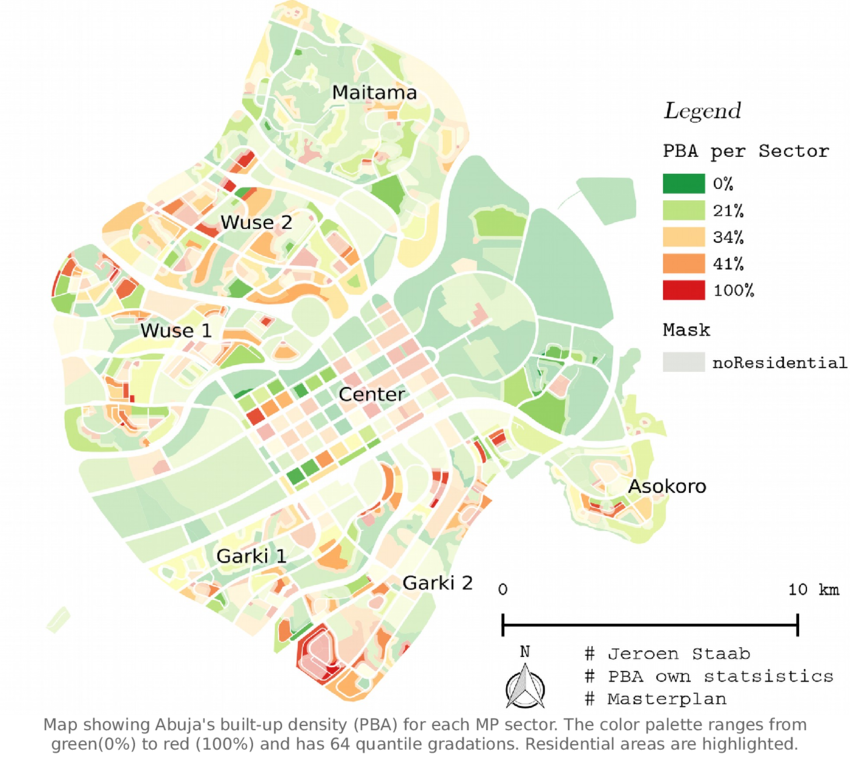
\includegraphics[width=\linewidth]{%
					images/abuja/Map-showing-Abujas-built-up-density-PBA-for-each-MP-sector-The-color-palette-ranges.png%
				}
				\caption{Abuja's built-up density (PBA), 2015\cite{ResearchGate:AbujaDensity}}
				\label{fig:images:abuja-density}
			\end{figure}
			
			The (first) railway line, connecting the central business district, the main station and the airport, was finalized 2018.
			
			
			\subsubsection{Today}
			
			Abuja is one of the fastest growing cities in the world. It grows between 20\% and 30\% per year. The development inside the planned area is more ore less following the master plan, but slums and sprawling suburbs are growing uncontrolled, spread all over the metropolitan region.
			
			\begin{table}[H]			
				\centering
				\caption{Facts}
				\label{table:abuja-facts}
				\begin{tabular}{|l|l|}
					\hline
					\textbf{Population}           & \textgreater 3 M \\
					\textbf{Urban density}        & 35 pop./ha \\
					\textbf{Metropolitan density} & 7 pop./ha \\
					\hline
				\end{tabular}
			\end{table}
			
			The density of the urban area is around 35 inhabitants per hectare and the overall density of the metropolitan region around 7 inhabitants.
			Abuja has a population of around 3 millions and it's expected that it will grow up to 5 million people to 2030.
			
			\begin{figure}[H]			
				\includegraphics[width=\linewidth]{%
					maps/abuja/2019.jpg%
				}
				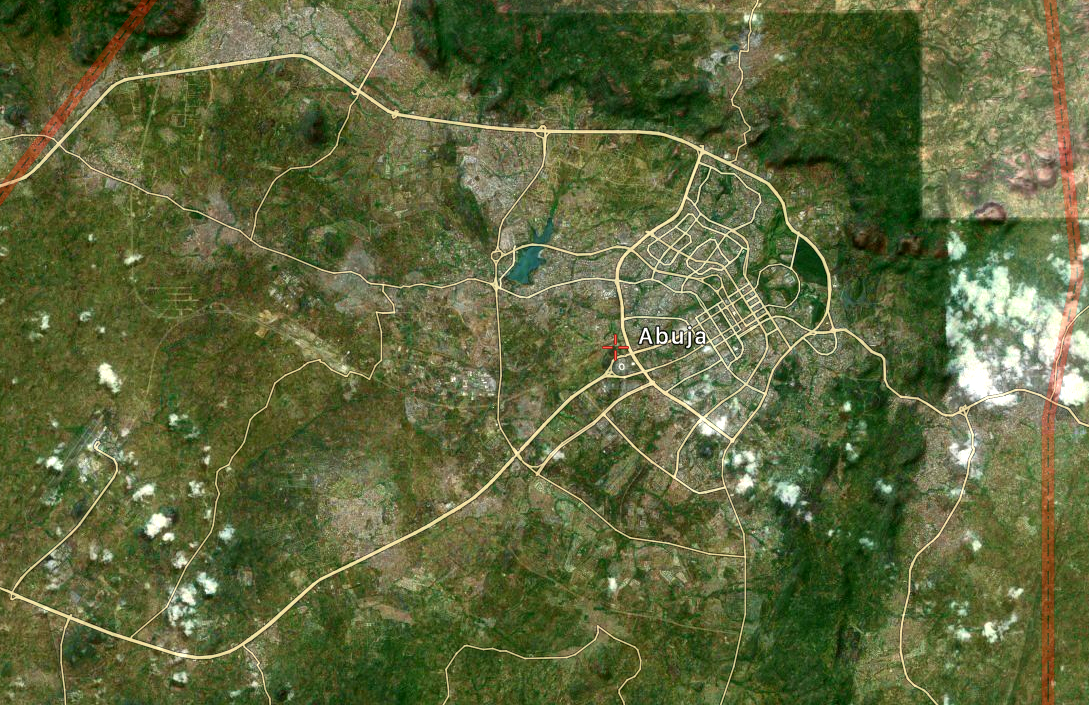
\includegraphics[width=\linewidth]{%
					images/abuja/2019-aerial.png%
				}
				\caption{Map\cite{OpenStreetMap:Abuja} and satellite image\cite{Satellites.pro:Abuja} of Abuja, 2019}
				\label{fig:map:abuja-map-satellite-2019}
			\end{figure}
			
			Slums are the fastest growing areas and are  filling open areas inside the planned areas.
			
			\begin{figure}[H]
				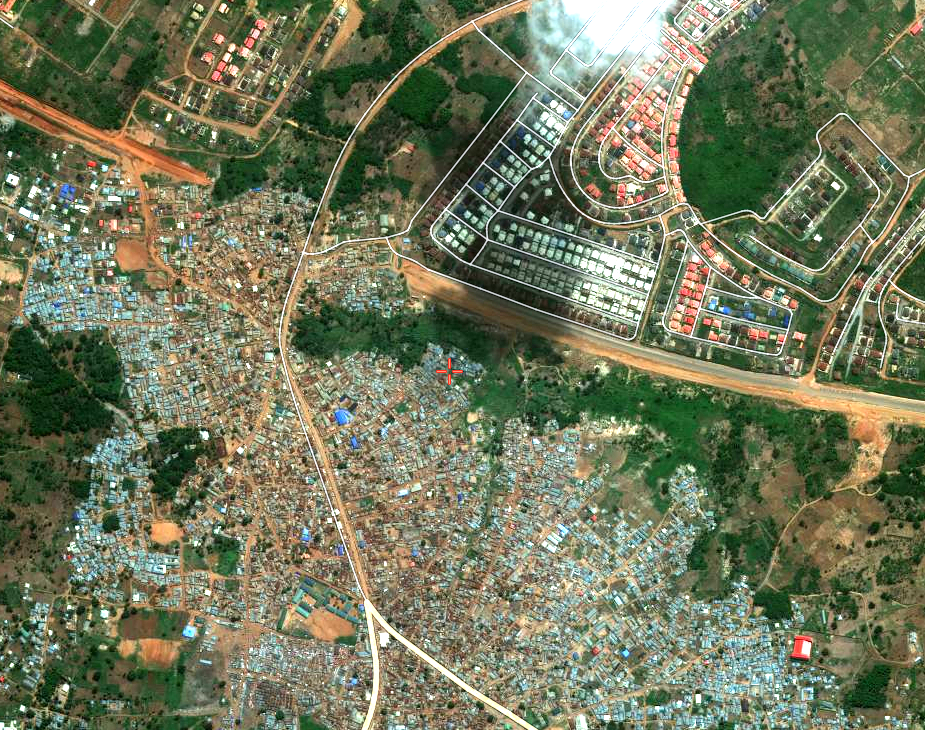
\includegraphics[width=\linewidth]{%
					images/abuja/slums.png%
				}
				\caption{Slums in Abuja (bottom), along with planned development (top right), 2019\cite{Satellites.pro:Abuja}}
				\label{fig:images:abuja-slums}
			\end{figure}
			
			Abuja has high capacity bus routes and many mini bus services. But not all districts are connected and the buses often do not stop at the official stops and are unreliable.
			
			\begin{figure}[H]
				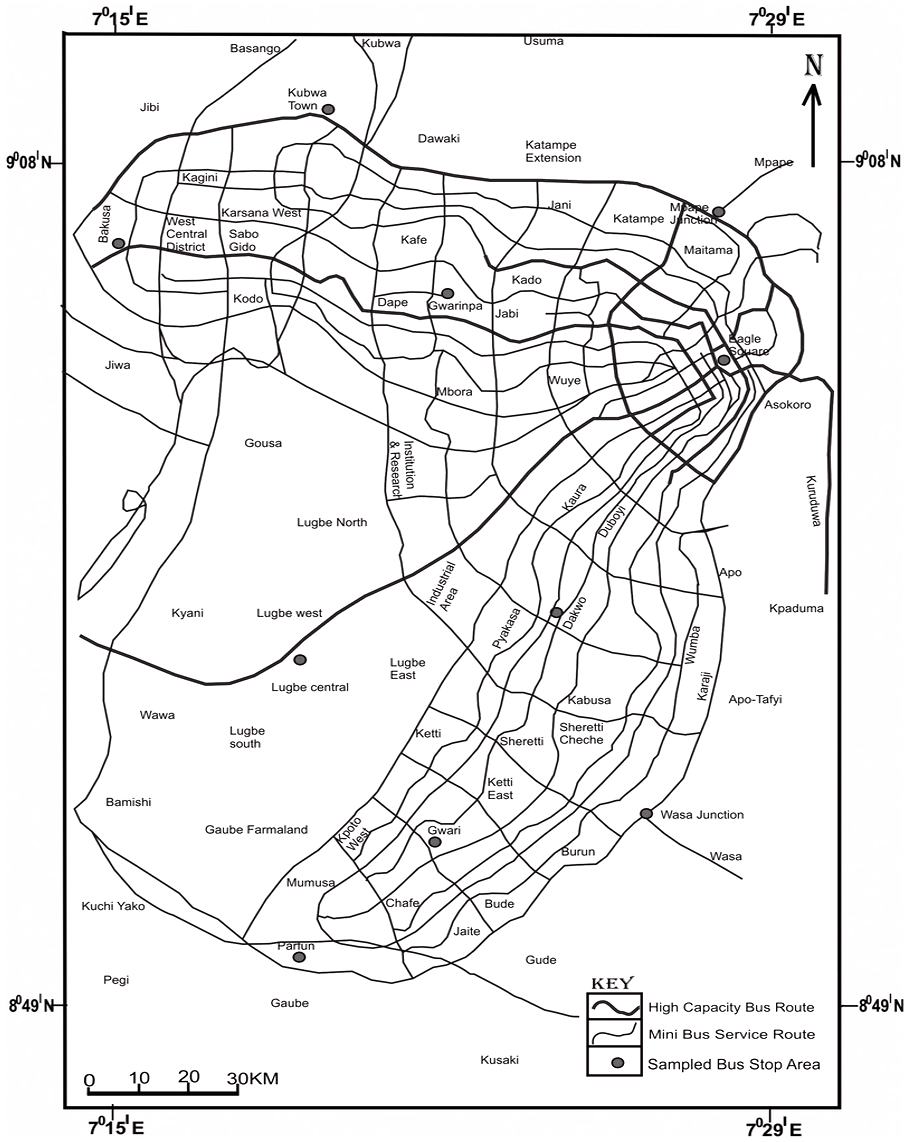
\includegraphics[width=\linewidth]{%
					maps/abuja/Bus-route-network-in-Federal-Capital-Territory-Abuja.png%
				}
				\caption{Abuja bus route network, 2014\cite{ResearchGate:AbujaBusRouteNetwork}}
				\label{fig:map:abuja-bus-route-network}
			\end{figure}
			
			The light rail line to the airport also links the main railway station and counts with several stations. But many of them are far away from the next districts. People need to walk long distances or drive to get there.
			
			The rest of the planned rail network is yet outstanding. The national trains arrive at the main station outside of Abuja, but do not get yet to the city center.
			
			Also the national railway network was not expanded like planned. Abuja is only connected to Kaduna in the north. Links to the south, east and west are planned but were not yet constructed.
			
			\begin{figure}[H]
				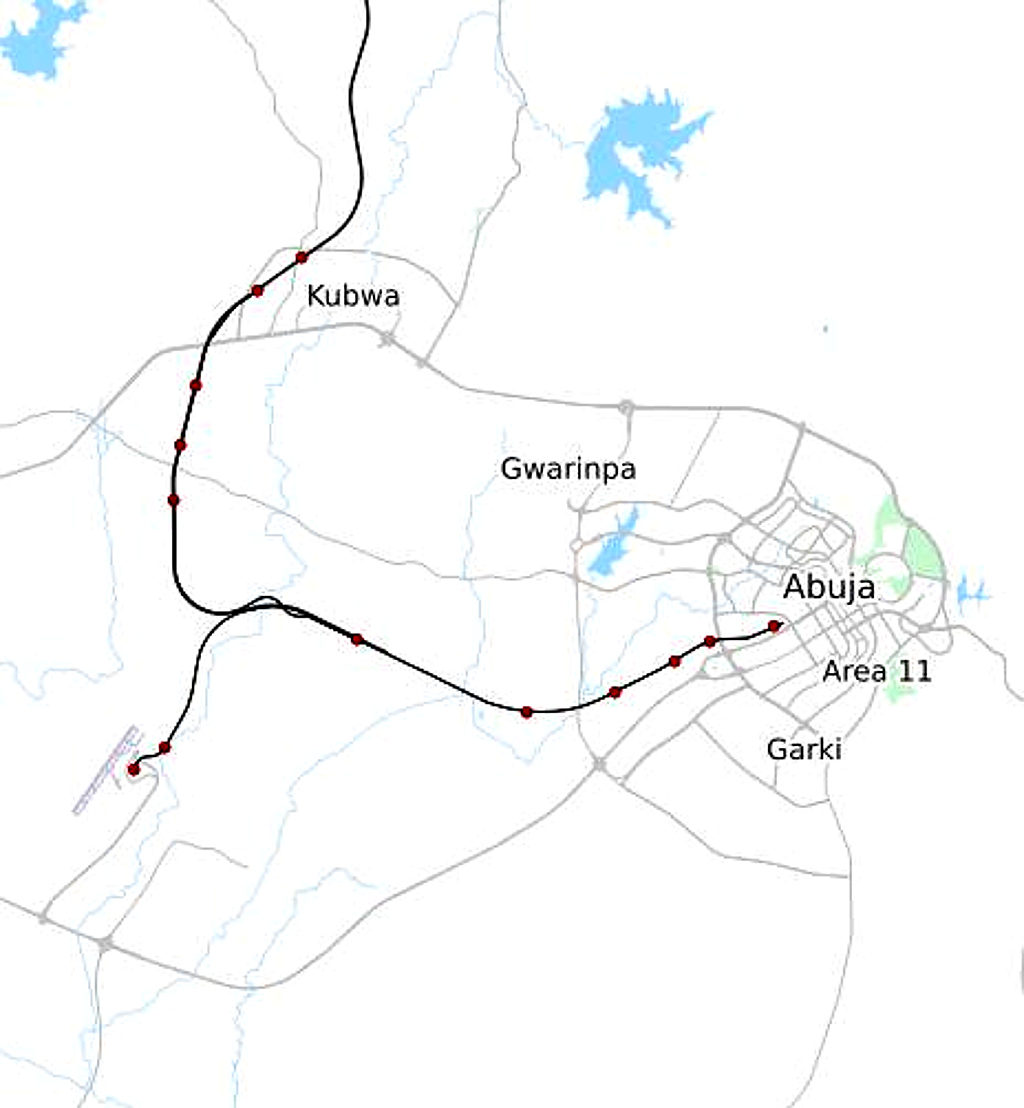
\includegraphics[width=\linewidth]{%
					maps/abuja/2019-rail-network.jpg%
				}
				\caption{Abuja rail and light rail network, 2019\cite{ResearchGate:AbujaBusRouteNetwork}}
				\label{fig:map:abuja-rail-network-2019}
			\end{figure}
			
			Abuja counts with a lot of pedestrian and cyclists. Especially the poor population can not afford to drive.
			The city does not count with bicycle infrastructure yet and the infrastructure is most car oriented.
			
			In the central business district, a lot of blocks are not developed yet, pedestrian links are missing and people need to walk long distances on highly transited arterials.
			
			\begin{figure}[H]
				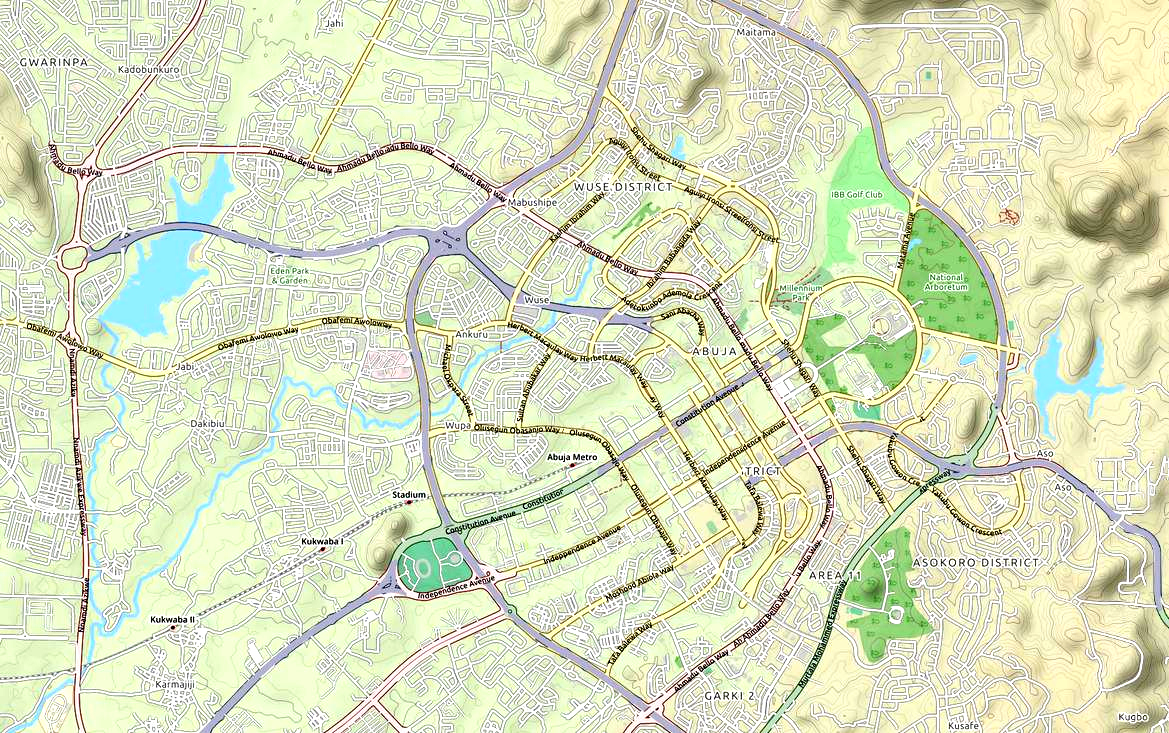
\includegraphics[width=\linewidth]{%
					maps/abuja/2019-cbc-cycle-infrastructure.jpg%
				}
				\caption{Abuja's (not existing) bicycle infrastructure in the city center, 2019\cite{OpenCycleMap:Abuja}}
				\label{fig:map:abuja-bicycle-map-2019}
			\end{figure}	
			
			
			\subsubsection{Roundup}
			
			


	\clearpage
	\section{Conclusion}

	
	\begin{comment}
	https://www.latex-tutorial.com/tutorials/table-of-contents/
	https://en.wikibooks.org/wiki/LaTeX/
	
https://en.m.wikipedia.org/wiki/Planned_community

https://de.wikipedia.org/wiki/La_Chaux-de-Fonds
Batavia, Indonesia, 17th century, https://en.m.wikipedia.org/wiki/Batavia,_Dutch_East_Indies
Ashdod, Israel, 1956,https://en.m.wikipedia.org/wiki/Ashdod
Kyoto, Japan, 794, https://en.m.wikipedia.org/wiki/Kyoto
Navi Mumbai, India, 1960, https://en.m.wikipedia.org/wiki/Navi_Mumbai
Adelaide, Australia, 1836, https://en.m.wikipedia.org/wiki/Adelaide
Washington D.C., USA, 1790, https://en.m.wikipedia.org/wiki/Washington,_D.C.

two figures in one line
\begin{figure}[h!]
  \centering
  \begin{subfigure}[b]{0.4\linewidth}
    \includegraphics[width=\linewidth]{coffee.jpg}
    \caption{Coffee.}
  \end{subfigure}
  \begin{subfigure}[b]{0.4\linewidth}
    \includegraphics[width=\linewidth]{coffee.jpg}
    \caption{More coffee.}
  \end{subfigure}
  \caption{The same cup of coffee. Two times.}
  \label{fig:coffee}
\end{figure}

\begin{itemize}
\item \blindtext
\item \blindtext
\end{itemize}
\begin{enumerate}
\item \blindtext
\item \blindtext
\end{enumerate}
\begin{description}
\item [Ant] \blindtext
\item [Elephant] \blindtext
\end{description}

@BOOK{DUMMY:1,
AUTHOR="John Doe",
TITLE="The Book without Title",
PUBLISHER="Dummy Publisher",
YEAR="2100",
}


	\end{comment}
	
	\clearpage
	\begin{strip}
		\begin{appendix}
			\bibliography{references} 
			\bibliographystyle{ieeetr}
		
			\listoffigures
		
			\listoftables
		\end{appendix}
	\end{strip}
\end{document}


